\documentclass[a4paper,12pt]{extreport}

\usepackage[T2A]{fontenc}
\usepackage[utf8]{inputenc}
\usepackage[english,russian]{babel}
\usepackage{tempora}
\usepackage{geometry}
\usepackage{setspace}
\usepackage{indentfirst}
\usepackage{graphicx}
\usepackage{float}
\usepackage{caption}
\usepackage{array}
\usepackage{longtable}
\usepackage{booktabs}
\usepackage{listings}
\usepackage{xcolor}
\usepackage{enumitem}
\usepackage{titlesec}
\usepackage[titles]{tocloft}
\usepackage[hidelinks]{hyperref}
\usepackage{fancyhdr}
\usepackage{lastpage}

\geometry{left=30mm,right=15mm,top=20mm,bottom=20mm}
\onehalfspacing
\setlength{\parindent}{1.25cm}
\setlength{\parskip}{0pt}
\setlist{nosep,wide=\parindent,labelsep=0.4em}
\setlist[itemize]{label=--}
\graphicspath{{images/}}

\titleformat{\chapter}[hang]
  {\normalfont\normalsize\bfseries\filright\hyphenpenalty=10000}
  {\thechapter}{0.5em}{}
\titleformat{name=\chapter,numberless}[block]
  {\normalfont\normalsize\bfseries\filcenter\hyphenpenalty=10000}
  {}{0pt}{}
\titleformat{\section}[hang]
  {\normalfont\normalsize\bfseries\filright\hyphenpenalty=10000}
  {\thesection}{0.5em}{}
\titleformat{\subsection}[hang]
  {\normalfont\normalsize\bfseries\filright\hyphenpenalty=10000}
  {\thesubsection}{0.5em}{}
\titlespacing{\chapter}{1.25cm}{0pt}{\baselineskip}
\titlespacing{name=\chapter,numberless}{0pt}{0pt}{\baselineskip}
\titlespacing{\section}{1.25cm}{\baselineskip}{\baselineskip}
\titlespacing{\subsection}{1.25cm}{\baselineskip}{0.5\baselineskip}

\renewcommand{\cftchapleader}{\cftdotfill{\cftdotsep}}
\renewcommand{\cftchapfont}{\normalfont}
\renewcommand{\cftchappagefont}{\normalfont}
\addto\captionsrussian{\renewcommand{\contentsname}{СОДЕРЖАНИЕ}}
\addto\captionsrussian{\renewcommand{\bibname}{СПИСОК ИСПОЛЬЗОВАННЫХ ИСТОЧНИКОВ}}
\makeatletter
\renewcommand{\@biblabel}[1]{#1.}
\makeatother

\captionsetup{labelsep=endash,justification=centering}
\captionsetup[table]{justification=raggedright,singlelinecheck=false,position=top}
\addto\captionsrussian{\renewcommand{\figurename}{Рисунок}}
\addto\captionsrussian{\renewcommand{\tablename}{Таблица}}

\fancypagestyle{plain}{%
  \fancyhf{}%
  \fancyfootoffset[L]{15mm}%
  \fancyfoot[C]{\thepage}%
  \renewcommand{\headrulewidth}{0pt}%
}
\pagestyle{plain}

\lstdefinestyle{code}{
  basicstyle=\ttfamily\normalsize,
  numbers=left,
  numberstyle=\tiny,
  numbersep=8pt,
  frame=single,
  xleftmargin=22pt,
  xrightmargin=4pt,
  framexleftmargin=18pt,
  breaklines=true,
  showstringspaces=false,
  tabsize=4,
  columns=fullflexible,
  inputencoding=utf8,
  extendedchars=true
}

\lstdefinestyle{logstyle}{
  basicstyle=\ttfamily\normalsize,
  numbers=left,
  numberstyle=\tiny,
  numbersep=7pt,
  xleftmargin=25pt,
  breaklines=true,
  breakatwhitespace=false,
  showstringspaces=false,
  showtabs=false,
  tabsize=2,
  columns=fullflexible,
  keepspaces=true,
  inputencoding=utf8,
  extendedchars=true,
  captionpos=t,
  abovecaptionskip=8pt,
  literate={×}{{$\times$}}1
           {«}{{\guillemotleft}}1 {»}{{\guillemotright}}1
           {–}{{\textendash}}1 {—}{{\textemdash}}1 {→}{{$\rightarrow$}}1
           {а}{{\char224}}1 {б}{{\char225}}1 {в}{{\char226}}1 {г}{{\char227}}1 {д}{{\char228}}1 {е}{{\char229}}1 {ё}{{\cyryo}}1 {ж}{{\char230}}1 {з}{{\char231}}1 {и}{{\char232}}1 {й}{{\char233}}1 {к}{{\char234}}1 {л}{{\char235}}1 {м}{{\char236}}1 {н}{{\char237}}1 {о}{{\char238}}1 {п}{{\char239}}1 {р}{{\char240}}1 {с}{{\char241}}1 {т}{{\char242}}1 {у}{{\char243}}1 {ф}{{\char244}}1 {х}{{\char245}}1 {ц}{{\char246}}1 {ч}{{\char247}}1 {ш}{{\char248}}1 {щ}{{\char249}}1 {ъ}{{\char250}}1 {ы}{{\char251}}1 {ь}{{\char252}}1 {э}{{\char253}}1 {ю}{{\char254}}1 {я}{{\char255}}1
           {А}{{\char192}}1 {Б}{{\char193}}1 {В}{{\char194}}1 {Г}{{\char195}}1 {Д}{{\char196}}1 {Е}{{\char197}}1 {Ж}{{\char198}}1 {З}{{\char199}}1 {И}{{\char200}}1 {Й}{{\char201}}1 {К}{{\char202}}1 {Л}{{\char203}}1 {М}{{\char204}}1 {Н}{{\char205}}1 {О}{{\char206}}1 {П}{{\char207}}1 {Р}{{\char208}}1 {С}{{\char209}}1 {Т}{{\char210}}1 {У}{{\char211}}1 {Ф}{{\char212}}1 {Х}{{\char213}}1 {Ц}{{\char214}}1 {Ч}{{\char215}}1 {Ш}{{\char216}}1 {Щ}{{\char217}}1 {Ы}{{\char219}}1 {Ь}{{\char220}}1 {Э}{{\char221}}1 {Я}{{\char223}}1
}

\newcommand{\code}[1]{\texttt{#1}}
\newcommand{\logfile}[2]{\lstinputlisting[style=logstyle,caption={#1}]{#2}}
\makeatletter
\newcommand{\gostappendix}[1]{%
  \clearpage
  \refstepcounter{chapter}%
  \def\@currentlabelname{#1}%
  \addcontentsline{toc}{chapter}{Приложение \thechapter{} (справочное) #1}%
  {\normalfont\normalsize\centering\hyphenpenalty=10000
    ПРИЛОЖЕНИЕ \thechapter\par
    (справочное)\par
    \vspace{0.5\baselineskip}%
    {\bfseries #1\par}}%
  \vspace{\baselineskip}%
}
\makeatother

% Структурный элемент отчёта: заголовок без номера, с записью в содержание.
\newcommand{\structel}[1]{%
  \clearpage\phantomsection\addcontentsline{toc}{chapter}{#1}%
  \chapter*{#1}}

\begin{document}

\begin{titlepage}
\singlespacing
\thispagestyle{empty}
\noindent\begin{minipage}{0.13\textwidth}
  
\includegraphics[width=\linewidth]{b_logo.png}
\end{minipage}%
\hfill%
\begin{minipage}{0.84\textwidth}
\centering\small\bfseries
Министерство науки и высшего образования Российской Федерации\\
Федеральное государственное автономное образовательное учреждение высшего образования\\
<<Московский государственный технический университет имени Н.~Э.~Баумана\\
(национальный исследовательский университет)>>\\
(МГТУ им. Н.~Э.~Баумана)
\end{minipage}

\vspace{0.3cm}
\noindent\rule{\linewidth}{2pt}
\vspace{0.7cm}

\noindent ФАКУЛЬТЕТ \underline{<<Информатика и системы управления>>}\\[0.5cm]
\noindent КАФЕДРА \underline{<<Программное обеспечение ЭВМ и информационные технологии, ИУ7>>}

\vfill
\begin{center}
{\Large\bfseries Лабораторная работа № 2}\\[0.4cm]
{\large по дисциплине}\\[0.2cm]
{\large\bfseries <<Программирование (специальные главы)>>}\\[1cm]
{\large\bfseries Сравнение больших языковых моделей при построении блок-схем алгоритма Дейкстры}
\end{center}
\vfill

\noindent\textbf{Студент:} \underline{Логинов Виктор Николаевич}\\[0.5cm]
\noindent\textbf{Группа:} \underline{СГН3-11М}\\[0.5cm]
\noindent\textbf{Преподаватель:} \underline{Строганов Юрий Владимирович}

\vfill
\begin{center}
Москва 2026
\end{center}
\end{titlepage}

\setcounter{page}{2}

\structel{РЕФЕРАТ}

Отчет \pageref{LastPage}~с., 9~рис., 1~табл., 1~источн., 6~прил.

{\noindent\raggedright\hyphenpenalty=10000\exhyphenpenalty=10000\relax
БЛОК-СХЕМЫ, ГОСТ 19.701--90, DRAW.IO, YED GRAPHML, БОЛЬШИЕ ЯЗЫКОВЫЕ МОДЕЛИ, АЛГОРИТМ ДЕЙКСТРЫ, СРАВНИТЕЛЬНЫЙ АНАЛИЗ\par}

Объектом исследования являются сохранённые ответы Qwen3.7-Plus, Korolev AI и DeepSeek, содержащие блок-схемы алгоритма Дейкстры в форматах draw.io XML и yEd GraphML.

Цель работы --- экспериментально оценить способность больших языковых моделей создавать редактируемые блок-схемы по исходному коду и требованиям ГОСТ 19.701--90.

Методами исследования служат единый исходный запрос, автоматическая проверка структуры XML, типов фигур, ссылок и геометрии, визуальная проверка в редакторах draw.io и yEd, а также учёт числа ответов до приёмки.

В результате работы получены шесть принятых схем; DeepSeek потребовал 6 ответов, Qwen3.7-Plus --- 11, Korolev AI --- 15. Наиболее устойчивые локальные исправления показал DeepSeek, Qwen3.7-Plus потребовал внешней координатной сетки, у Korolev AI отмечены регрессии текста и логики.

Область применения --- подготовка учебной и технической документации с помощью больших языковых моделей.

\tableofcontents

\chapter*{ПЕРЕЧЕНЬ СОКРАЩЕНИЙ И ОБОЗНАЧЕНИЙ}
\addcontentsline{toc}{chapter}{ПЕРЕЧЕНЬ СОКРАЩЕНИЙ И ОБОЗНАЧЕНИЙ}

В настоящем отчёте о лабораторной работе применяют следующие сокращения и обозначения.

\noindent
\begin{tabular}{@{}l@{\quad---\quad}p{0.72\linewidth}@{}}
БЯМ & большая языковая модель \\
ЕСПД & Единая система программной документации \\
GraphML & формат описания графов на основе XML \\
LLM & большая языковая модель (large language model) \\
PDF & формат переносимого документа \\
XML & расширяемый язык разметки
\end{tabular}

\begingroup
\titlespacing{name=\chapter,numberless}{0pt}{-8pt}{0.4\baselineskip}
\chapter*{ВВЕДЕНИЕ}
\addcontentsline{toc}{chapter}{ВВЕДЕНИЕ}
\endgroup

Цель работы --- экспериментально оценить способность больших языковых моделей создавать редактируемые блок-схемы алгоритма по исходному коду и формальным требованиям ГОСТ 19.701--90~\cite{gost19701}. Модель должна одновременно сохранить логику алгоритма, сформировать корректный XML конкретного редактора и выполнить пространственную компоновку элементов.

В исследовании сопоставлены Qwen3.7-Plus, Korolev AI и DeepSeek. Каждой модели передавался одинаковый исходный запрос. Требовалось получить две схемы алгоритма Дейкстры: реализацию Python в формате draw.io XML и реализацию C++ в формате yEd GraphML.

Результат проверялся на двух уровнях: автоматически по структуре XML и фактически после открытия в соответствующем редакторе. Количество ответов до приёмки и необходимость задавать точные координаты использованы как показатели практической пригодности модели.

Актуальность работы обусловлена тем, что генерация текста программы и генерация редактируемой инженерной диаграммы предъявляют к большим языковым моделям (БЯМ) различные требования. В программном коде основная часть результата задаётся последовательностью символов и может быть проверена компилятором или интерпретатором. В блок-схеме, помимо логической правильности, необходимо обеспечить пространственное расположение фигур, корректное подключение линий к портам, отсутствие пересечений и однозначную связь подписей с ветвями условий. Формально допустимый XML при этом может отображаться неудовлетворительно и не выполнять главную функцию схемы --- облегчать чтение алгоритма.

Объектом исследования являются последовательности ответов трёх БЯМ при решении одной и той же задачи. Предмет исследования --- качество создаваемых ими XML-описаний блок-схем и устойчивость последующих исправлений. Под устойчивостью понимается способность модели устранить указанный дефект, сохранив ранее корректные элементы, текст условий и структуру управляющего потока.

Для достижения поставленной цели решались следующие задачи: формулировалась единая исходная постановка; фиксировались все ответы моделей; из ответов извлекались файлы draw.io и GraphML; выполнялась автоматическая проверка XML, связей и геометрии; формировались уточняющие запросы; результаты открывались в целевых редакторах; после принятия обеих схем сопоставлялись количество итераций, характер дефектов и объём необходимого ручного сопровождения.

Практический результат работы состоит не только в получении шести редактируемых схем. Сформирован воспроизводимый процесс проверки генеративных результатов, в котором автоматический анализ и визуальная экспертиза дополняют друг друга. Такой процесс может применяться при подготовке учебной документации, технических схем и иных структурированных графических материалов, создаваемых с помощью БЯМ.

\chapter{Аналитическая часть}

\section{Описание задачи и выбранных инструментов}

\subsection{Исходный алгоритм}

В качестве основы использован алгоритм Дейкстры для графа, заданного матрицей весов. Программы принимают число вершин, матрицу, начальную и конечную вершины. После проверки индексов выполняются инициализация массивов расстояний и предшественников, выбор непосещённой вершины с минимальной меткой, релаксация рёбер и восстановление маршрута.

Для построения блок-схемы алгоритм был разложен на логически завершённые операции. Внешний цикл включает выбор текущей непосещённой вершины, проверку возможности дальнейшего движения и пометку выбранной вершины как посещённой. Внутренний цикл перебирает соседей, отбрасывает отсутствующие или уже обработанные рёбра, вычисляет длину нового пути и при необходимости обновляет расстояние и предшественника. После завершения поиска отдельно проверяется достижимость конечной вершины, затем маршрут восстанавливается обратным проходом по массиву предшественников.

Такое разложение задаёт обязательный управляющий каркас схемы. Потеря любой из проверок меняет поведение программы: например, отсутствие условия недостижимости приводит к попытке восстановить несуществующий маршрут, а неверное направление возврата внутреннего цикла нарушает перебор соседей. Поэтому логическая эквивалентность исходному коду оценивалась независимо от внешней аккуратности изображения.

Версия C++ дополнительно содержит проверку
\begin{center}
\code{distance[current] <= INF - weight}.
\end{center}
Она предотвращает переполнение целого типа. Соответствующий ромб должен присутствовать только в C++-схеме.

Различие между реализациями принципиально для эксперимента: модель не должна механически копировать один набор блоков в оба формата. От неё требовалось распознать специфическую для C++ защиту и отразить её отдельным условием, сохранив при этом общий алгоритмический каркас. Это позволяло проверить не только способность рисовать фигуры, но и понимание связи между исходным кодом и его графическим представлением.

\subsection{Форматы и редакторы}

Каждая модель должна была вернуть два редактируемых файла:

\begin{enumerate}[label=\arabic*)]
  \item \code{python\_gost.drawio} --- несжатый XML draw.io с одной страницей~<<Python~ГОСТ>>;
  \item \code{cpp\_gost.graphml} --- yEd GraphML с ориентированной схемой <<C++ ГОСТ>>.
\end{enumerate}

Начало и конец оформлялись терминаторами, ввод и вывод --- параллелограммами, вычисления --- прямоугольниками, условия --- ромбами. Все переходы должны быть направленными и ортогональными, а подписи <<Да>> и <<Нет>> --- однозначно относиться к соответствующим ветвям.

Формат draw.io хранит диаграмму как набор ячеек \code{mxCell} с геометрией \code{mxGeometry}, стилями фигур и маршрутными точками рёбер. GraphML редактора yEd использует элементы узлов и рёбер совместно с расширениями yWorks, где отдельно задаются геометрия узла, тип фигуры, область подписи, порты и путь ребра. В обоих случаях XML может быть синтаксически корректным, даже если линия проходит через соседний блок или подпись отображается за пределами ромба.

Редактируемый формат был выбран намеренно. Растровое изображение могло бы выглядеть аккуратно, но не позволило бы проверить внутреннюю структуру, связи и пригодность к последующему изменению. XML-файл, напротив, даёт возможность сопоставлять версии, находить конкретные рёбра по идентификаторам и автоматически проверять часть требований до открытия редактора.

\section{Характеристика используемых БЯМ}

\subsection{Qwen3.7-Plus}

Qwen использовался без авторизации и без входа в учётную запись. Модель сразу формировала оба XML-файла и на поздних шагах достаточно точно выполняла локальные изменения идентификаторов, координат и портов. Основной недостаток проявился в пространственном планировании: синтаксически правильные схемы дважды оказались визуально неприемлемыми.

Сильной стороной Qwen оказалась работа с уже определённой структурой: когда запрос содержал конкретные идентификаторы, координаты и стороны входа, модель обычно изменяла нужные элементы без полного переписывания файлов. Однако при свободной компоновке она недооценивала ширину текста, объединяла независимые маршруты в один коридор и создавала геометрически допустимые, но плохо читаемые связи. Поэтому качество итоговой версии в значительной степени определялось детализацией внешнего задания.

\subsection{Korolev AI}

Korolev AI создавал редактируемые XML, но показал низкую устойчивость исправлений. При устранении геометрического дефекта модель могла изменить правильный текст или повредить условие. Совмещённая генерация двух файлов привела к обрыву ответа и последующему переполнению контекста старого диалога.

Для этой модели особенно заметно влияние длины диалога. Накопление полных XML-версий увеличивало контекст, а попытка продолжить оборванный ответ завершилась технической ошибкой. После разделения форматов работа стала управляемее, но локальные исправления всё равно сопровождались регрессиями: менялись операторы сравнения, подписи и маршруты, не упомянутые в корректирующем запросе.

\subsection{DeepSeek}

DeepSeek завершил цепочку за меньшее число ответов. Его исходная схема draw.io оказалась ближе к приемлемой. Однако GraphML также потребовал явного центрирования подписей и разведения длинных коридоров. Общая переработка на раннем шаге ухудшила draw.io, после чего исправления выполнялись раздельно.

Наблюдение показывает, что меньшая длина цепочки не означает отсутствия ошибок. Преимущество DeepSeek проявилось в более удачной исходной компоновке и более быстром переходе к локальным исправлениям. После отказа от одновременной переработки двух форматов модель достаточно последовательно довела каждый файл до принятого состояния.

\section{Сравнительный анализ выбранных БЯМ}

Все три сервиса способны формировать машинно читаемый XML, но это не гарантирует качественной диаграммы. Qwen лучше Korolev AI воспроизводил поздние точечные изменения, DeepSeek потребовал меньше итераций, а Korolev AI чаще создавал регрессии и технические сбои.

До эксперимента нельзя было считать ни одну модель заведомо подходящей: проверяемые свойства включают не только синтаксис, но и логику, совместимость редактора, геометрию и визуальную читаемость. Поэтому окончательное сравнение выполнялось по сохранённым цепочкам ответов.

Для предварительного сравнения были выделены четыре группы критериев. Первая характеризует смысловую корректность: сохранение всех ветвей алгоритма и соответствие Python- и C++-версий исходному коду. Вторая относится к формату: валидность XML, корректность ссылок и возможность открыть файл в целевом редакторе. Третья описывает визуальное качество: размеры фигур, центрирование, ортогональность, отсутствие наложений и читаемость длинных связей. Четвёртая отражает практическую эффективность: число ответов, устойчивость локальных правок и необходимость задавать модели низкоуровневую геометрию.

Ожидалось, что автоматические проверки надёжно выявят структурные ошибки, но не смогут полностью заменить визуальную оценку. Также предполагалось, что модели будут различаться не столько способностью однажды сформировать XML, сколько стоимостью доведения первоначального результата до состояния, пригодного для использования.

\chapter{Конструкторский раздел}

\section{Процесс взаимодействия с моделями}

Всем участникам передавалась одна постановка с одинаковыми исходными программами и требованиями к форматам. Начальный запрос не адаптировался под сильные и слабые стороны конкретной модели. Каждый ответ сохранялся без изменений, после чего файлы извлекались в отдельный каталог итерации и проходили полный контроль.

Единообразие начального запроса необходимо для сопоставимости. Если одной модели заранее сообщить координаты всех блоков, а другой предоставить только описание алгоритма, число последующих исправлений будет отражать различия постановок, а не возможностей моделей. Поэтому исходные условия, код и критерии приёмки сохранялись одинаковыми, а уточнения формировались только на основе реально обнаруженных дефектов.

Если ответ разделял два файла между сообщениями, каждое фактически полученное сообщение учитывалось как отдельная итерация. Для Korolev AI после обрыва крупного ответа форматы пришлось разделить на два независимых направления, однако принцип последовательного учёта сохранился.

Для каждой итерации сохранялись исходный текст ответа, извлечённые файлы, результаты автоматических проверок и следующий корректирующий запрос. Такой журнал позволяет восстановить причинно-следственную связь: какое замечание получила модель, что именно она изменила и появились ли побочные дефекты. Итоговая версия не подменяла предыдущие файлы до завершения полного контроля.

Процесс взаимодействия представлял собой цикл: генерация --- извлечение --- автоматическая проверка --- открытие в редакторе --- фиксация дефектов --- корректирующий запрос. Цикл завершался отдельно для каждой модели только после принятия обеих диаграмм. Благодаря этому число ответов учитывает фактическую стоимость получения полного результата, а не первой синтаксически корректной версии.

\section{Построение исправляющего промта}

Корректирующий запрос составлялся только по обнаруженным дефектам. На ранних шагах использовались описательные требования: центрировать текст, убрать диагонали, развести длинные линии. Когда этого оказалось недостаточно, запросы стали содержать идентификаторы рёбер, стороны портов, точные размеры и координаты коридоров.

Исправляющий промт включал четыре части: перечень элементов, которые разрешено менять; описание наблюдаемого дефекта; проверяемое требование к новому состоянию; запрет на изменение остального содержимого. Для геометрических ошибок дополнительно задавались точки входа и выхода, минимальные интервалы между блоками и отдельные коридоры для длинных возвратов. Для текстовых регрессий указывалась точная строка или XML-представление специальных символов.

После каждой новой версии проверялся весь файл. Такой порядок необходим, поскольку модели неоднократно исправляли заданный элемент и одновременно создавали регрессию в другой части схемы.

Практика показала постепенный переход от смыслового диалога к редактированию XML по спецификации. Пока запрос звучал как <<сделать схему аккуратнее>>, модель самостоятельно выбирала компоновку и могла повторить прежний тип ошибки. Когда задавались идентификаторы, координаты и неизменяемые области, вероятность точного исправления возрастала, но доля творческой работы модели уменьшалась. Этот переход сам по себе является значимым результатом: высокое качество финального файла не всегда означает высокую самостоятельность БЯМ.

Полная перекомпоновка применялась только тогда, когда локальные правки переставали улучшать читаемость. Для Qwen такой момент наступил после второй ручной браковки: накопленные коридоры и пересечения нельзя было надёжно устранить отдельными смещениями. Новая компоновка задала центральную ось основного потока и независимые области для циклов и аварийных выходов.

\section{Проектирование набора проверок}

Автоматическая проверка включала:

\begin{itemize}
  \item синтаксический разбор XML;
  \item уникальность идентификаторов и существование \code{source}/\code{target};
  \item наличие единственного начала и общего конца;
  \item соответствие типов фигур операциям алгоритма;
  \item число блоков, наконечники и подписи условных ветвей;
  \item маршрутные точки и очевидные пересечения линий с чужими узлами;
  \item наличие отдельной защиты от переполнения только в C++.
\end{itemize}

После автоматического контроля пользователь открывал файлы в draw.io и yEd. Проверялись фактическое центрирование текста, размеры фигур, читаемость подписей, видимость наконечников, отсутствие наложений и возможность проследить каждую связь.

Проверки были разделены на три уровня. На синтаксическом уровне устанавливалось, что XML разбирается и содержит требуемые пространства имён. На структурном уровне проверялись идентификаторы, ссылки, типы фигур, количество входов и выходов и наличие обязательных ветвей. На геометрическом уровне анализировались прямоугольники узлов, точки маршрутов и пересечения с чужими фигурами. Последний уровень оставался приближённым, поскольку фактический рендеринг зависит от настроек конкретного редактора.

Критерием автоматического прохождения считалось отсутствие обнаруженных нарушений на всех трёх уровнях. Критерием окончательного принятия являлась возможность открыть файл, прочитать все подписи и непрерывно проследить любой путь от начала до общего терминатора. Таким образом, автоматический статус \code{PASS} рассматривался как допуск к ручной проверке, а не как окончательное доказательство качества.

\section{Codex как внутренний контроллер работы и приёмки}

Внутренним контроллером экспериментального процесса с Qwen3.7-Plus, Korolev AI и DeepSeek выступал Codex. Он организовывал обработку ответов, проверку схем, подготовку обратной связи и техническую приёмку каждой итерации. Исследуемые модели генерировали блок-схемы по исходному и уточняющим запросам. Codex сохранял ответы, извлекал два обязательных файла, связывал их с номером итерации и определял следующий шаг работы по результатам проверок.

Первичный контроль охватывал полноту ответа и возможность разобрать XML. Затем Codex проверял идентификаторы узлов и рёбер, ссылки между ними, обязательные ветви исходного алгоритма, типы фигур и текст условий. На геометрическом этапе сопоставлялись координаты блоков, порты, маршрутные точки и пересечения с чужими фигурами. Исходный ответ, извлечённые файлы и результаты контроля сохранялись в отдельных каталогах одной итерации, что обеспечивало прослеживаемость решения о её принятии или отклонении.

При обнаружении дефекта Codex сопоставлял XML с ограничениями задачи и предыдущим артефактом, фиксировал причину отклонения и составлял следующий запрос. В запрос включались идентификаторы проблемных элементов, допустимые изменения, координатные ограничения и требования к сохранению остальных элементов. После получения нового ответа Codex проверял выполнение запрошенной правки и повторно контролировал весь файл, включая ранее исправленные участки. Таким способом он отслеживал регрессии текста, логики и компоновки на протяжении всей цепочки.

В десятой итерации Qwen координатная проверка выявила пересечение двух ветвей в точке $(330, 1110)$ после перекомпоновки. Для одиннадцатой итерации запрос задал два раздельных правых коридора по $x=1060$ и $x=1120$. Повторная проверка подтвердила устранение этого пересечения и сохранение раздельных входов в условие выбора соседа. В пятнадцатой итерации Korolev AI контроль XML подтвердил, что закодированные числовыми ссылками операторы \code{==} восстановлены в подписи узла \code{n7}, а остальное содержимое GraphML совпадает с предыдущей версией.

Для визуального этапа пользователь открывал файлы в draw.io и yEd и сообщал результаты просмотра. Codex включал эту обратную связь в общий протокол приёмки, связывал замечания с конкретной версией и формировал требования к следующему ответу. Так, две автоматически прошедшие проверку версии Qwen были отклонены после пользовательского просмотра. Для продолжения работы Codex учитывал выявленные проблемы отображения и повторно проверял очередное исправление.

Codex принимал итоговое техническое решение по комплектности обоих форматов, результатам повторного контроля XML и геометрии, а также зафиксированному просмотру в редакторах. Он сохранял принятые экземпляры в каталогах \code{final}, завершая цикл приёмки соответствующей версии.

\chapter{Технологическая часть}

\section{Выбор языка и среды программирования}

Исходные реализации заданы на Python и C++. Для схем использованы форматы draw.io XML и yEd GraphML. Проверка выполнялась средствами Python и PowerShell: XML разбирался программно, координаты узлов и маршрутных точек сопоставлялись с геометрией блоков, а версии сравнивались побайтово и по структуре.

Отчёт подготовлен в LaTeX и собран pdfLaTeX. Для визуального контроля PDF преобразовывался в изображения средствами Poppler. Такой набор инструментов обеспечивает воспроизводимый контроль исходных данных, ответов моделей и готового отчёта.

Python выбран для проверяющих сценариев благодаря стандартным средствам разбора XML и удобству обработки коллекций узлов, рёбер и координат. PowerShell применялся для организации каталогов итераций, вычисления контрольных сумм и вызова проверок в среде Windows. Разделение ролей позволяло использовать Python для содержательного анализа, а командную оболочку --- для воспроизводимой последовательности операций над файлами.

LaTeX использован не только как средство набора текста. Он обеспечивает единую нумерацию разделов, таблиц, рисунков и приложений, автоматически формирует оглавление и позволяет включать исходные программы без ручного форматирования каждой строки. Рендеринг страниц в PNG применялся для контроля тех дефектов, которые невозможно обнаружить по журналу компиляции: неудачных переносов, переполнения таблиц, слишком мелких рисунков и нарушения визуальной иерархии.

Организация материалов построена вокруг неизменяемых исходных ответов. Для каждой модели предусмотрены каталоги запросов, последовательных итераций и финальных файлов. Внутри итерации раздельно сохраняются исходный ответ, извлечённые артефакты и отчёт проверки. Такая структура исключает потерю промежуточных версий и позволяет повторить анализ после изменения критериев.

\section{Реализация программного обеспечения}

\subsection{Решение Qwen3.7-Plus}

Итоговый draw.io содержит 17 блоков и 21 ребро. Итоговый GraphML содержит 18 узлов и 23 ребра. Основной поток расположен по центральной оси, вычисления внутреннего цикла вынесены в правую колонку, а длинные переходы используют отдельные коридоры. Оба файла приняты из итерации 11.

В принятой компоновке ветви ошибочного ввода и отсутствующего маршрута не пересекают основной вычислительный поток. Возврат внутреннего цикла приходит к условию по отдельному входу и не сливается с линией первичного входа. Подписи условных переходов размещены рядом с выходами из ромбов, что уменьшает вероятность прочитать длинную ветвь как продолжение соседнего условия.

Важно, что итоговое качество было достигнуто не за счёт первой генерации Qwen. К одиннадцатой итерации модель получила почти полное внешнее описание топологии: положение колонок, размеры фигур, стороны портов и координаты коридоров. Поэтому файл демонстрирует способность модели точно реализовать спецификацию, но не подтверждает столь же высокую способность самостоятельно спроектировать читаемую схему.

\subsection{Решение Korolev AI}

Итоговый draw.io содержит 19 блоков и 24 ребра и принят из итерации 12. Итоговый GraphML содержит 20 узлов и 25 рёбер и принят из итерации 15. Различие в числе блоков связано с более подробным отображением внутреннего цикла.

Финальные версии Korolev AI сохраняют корректную логику, однако путь к ним включал многократное восстановление ранее исправленных элементов. Для GraphML отдельно задавались размеры всех областей подписей и расстояния между боковыми узлами. Длинные возвраты были разведены по нескольким вертикальным коридорам, чтобы избежать прохождения через блок внутреннего цикла.

Последняя правка GraphML была минимальной: требовалось восстановить операторы равенства в одном условии. Обычное текстовое представление ранее изменялось моделью, поэтому символы были переданы числовыми XML-ссылками. Этот эпизод показывает, что даже локальное исправление текста может требовать знания особенностей формата и не сводится к естественно-языковой инструкции.

\subsection{Решение DeepSeek}

Файл draw.io принят из итерации 04, GraphML --- из итерации 06. Для yEd использованы явные прямоугольники подписей с математическим центрированием, а длинные возвраты разведены по отдельным координатным коридорам.

Схема draw.io сохранила удачную основу первой версии и была доведена локальными изменениями. Для GraphML потребовалось явно задать внутренние области \code{NodeLabel}, поскольку стандартного указания центрирования оказалось недостаточно для стабильного отображения длинных подписей. Отдельное размещение меток ветвей исключило их наложение на линии и соседние ромбы.

DeepSeek быстрее других моделей перешёл к принятому результату, но этот результат также основан на итерационном контроле. После неудачной общей переработки было принято решение больше не изменять оба формата одновременно. Разделение задачи уменьшило риск того, что улучшение yEd-схемы ухудшит уже близкую к принятой draw.io-компоновку.

\section{Протоколы взаимодействия с БЯМ}

Исходные запросы, ответы и корректирующие запросы приведены в приложениях~\ref{app:qwen}, \ref{app:korolev} и \ref{app:deepseek}. Исходный код приведён в приложениях~\ref{app:python} и \ref{app:cpp}, состав электронных материалов --- в приложении~\ref{app:electronic}.

\subsection{Протокол Qwen3.7-Plus}

Зафиксировано 11 ответов. Автоматически корректные итерации 05 и 08 были отклонены после открытия в редакторах. Итерации 09--11 выполнили полную перекомпоновку и три последовательных локальных исправления.

В первых ответах преобладали ошибки маршрутизации: линии пересекали фигуры, а GraphML использовал некорректные точки подключения. После устранения структурных дефектов проявились проблемы рендеринга --- текст выходил за границы блоков, условия имели неверную форму, а некоторые стрелки визуально не доходили до общего конца. Вторая автоматически успешная версия была отклонена уже не из-за отдельных пересечений, а из-за общей нечитаемости взаимосвязей.

Перекомпоновка девятой итерации стала поворотной точкой: вместо продолжения локальных смещений была заново задана пространственная архитектура. Десятая и одиннадцатая итерации устраняли уже конкретные дефекты новой схемы. Это объясняет, почему Qwen занял промежуточное место по числу ответов, но потребовал значительного объёма проектирования со стороны пользователя.

\subsection{Протокол Korolev AI}

Зафиксировано 15 итераций. В цепочку вошли неполный ответ, ошибка HTTP 400 при переполнении контекста и раздельные диалоги для двух форматов. Принятые результаты получены в итерациях 12 и 15.

Основной источник дополнительных итераций --- низкая локальность изменений. Модель могла выполнить требуемое перемещение блока, но одновременно изменить подпись или вернуть ранее устранённое пересечение. Из-за этого каждая новая версия требовала не выборочной проверки исправленного участка, а полного повторного анализа обоих файлов.

Технические ограничения диалога также повлияли на результат. Полные документы XML занимали значительный объём контекста. После обрыва сообщения попытка продолжить старую цепочку превысила доступный лимит. Разделение форматов и новые диалоги позволили завершить работу, но увеличили организационные затраты и потребовали переносить в каждый новый запрос полный набор актуальных ограничений.

\subsection{Протокол DeepSeek}

Зафиксировано 6 ответов. После ухудшения общей компоновки изменения были разделены по форматам. Draw.io завершён раньше, дальнейшие ответы содержали только GraphML.

В отличие от Korolev AI, DeepSeek реже повреждал уже исправленный текст и быстрее реагировал на явные требования к областям подписей. Основные усилия пришлись на геометрию yEd, где требовалось согласовать координаты узлов, меток и длинных обратных связей. После разделения форматов цепочка стала последовательной и завершилась без повторной полной перекомпоновки.

Протокол DeepSeek показывает преимущество раннего сохранения удачной основы. Вместо полного переписывания относительно качественной draw.io-схемы эффективнее оказалось вернуть её и вносить небольшие проверяемые изменения. Этот подход сократил число новых регрессий и сохранил читаемую композицию.

\chapter{Исследовательский раздел}

\section{Объекты исследования и методика оценки}

Объектами исследования являются сохранённые последовательности ответов трёх БЯМ и шесть итоговых редактируемых диаграмм. Оценивались полнота ответа, корректность управляющего потока, совместимость XML, качество визуальной компоновки, устойчивость исправлений и число ответов до принятия обоих файлов.

Эксперимент содержит одну последовательную цепочку на модель. Поэтому число итераций характеризует конкретный наблюдаемый процесс и не является статистической вероятностью успеха нового независимого запроса.

Единицей наблюдения являлся фактически полученный ответ модели, а не число отправленных пользовательских сообщений. Такой способ учёта важен для длинных результатов: если модель разбивала два файла на отдельные ответы или обрывала генерацию, каждый ответ увеличивал фактическую продолжительность работы и объём последующей проверки. Итоговой точкой считалось принятие обоих форматов, поскольку получение только одной корректной схемы не выполняло исходное задание.

Качественные показатели оценивались по журналу дефектов. Ошибки были сгруппированы в логические, форматные, геометрические, типографические и технические. Логические ошибки меняют алгоритм; форматные препятствуют разбору или открытию; геометрические создают пересечения и неоднозначные маршруты; типографические ухудшают чтение подписей; технические связаны с обрывом ответа или ограничением контекста. Такое разделение позволяет анализировать не только количество итераций, но и причины их появления.

Итоговая оценка не сводилась к внешней привлекательности. Схема признавалась пригодной, если она сохраняла алгоритм, открывалась как редактируемый документ, использовала требуемые обозначения и позволяла без догадок проследить все основные и аварийные пути. Визуальная аккуратность рассматривалась как функциональное требование, поскольку нечитаемая связь фактически скрывает логику программы.

\section{Ход исследования и анализ взаимодействия}

\subsection{Qwen3.7-Plus}

Первый ответ правильно передавал основной управляющий поток, но рёбра пересекали блоки, порты GraphML выходили за границы узлов, а подписи использовали неподходящую модель размещения.

На раннем этапе Qwen демонстрировал хорошее понимание последовательности вычислений. В схемах присутствовали проверка входных вершин, инициализация, два уровня цикла, обработка недостижимости и восстановление маршрута. Следовательно, основная проблема заключалась не в восстановлении алгоритма по коду, а в преобразовании этого алгоритма в пространственно организованный документ.

К пятой итерации автоматические проверки перестали находить нарушения. Фактическое открытие выявило выход текста, отсутствие центрирования, неверные формы условий, косые линии и плохо видимые пути к общему терминатору. После исправлений восьмая итерация также прошла автоматический контроль, но пользователь вновь отклонил её: рёбра сливались, подписи были двусмысленны, связи не прослеживались.

Две ручные браковки показывают границу применимости координатного анализатора. Он мог определить, что маршрутная точка не лежит внутри чужого прямоугольника, но не мог надёжно оценить визуальное слияние параллельных рёбер, близость подписи к конкретной ветви и реальную внутреннюю область текста после рендеринга. Поэтому автоматическое отсутствие пересечений ещё не означало, что читатель однозначно восстановит граф переходов.

Девятая итерация полностью перекомпоновала обе схемы по заданной координатной сетке. Десятая исправила подписи и совпадающие входные сегменты, одиннадцатая --- последнее пересечение длинных ветвей. После этого пользователь принял оба файла.

Qwen нельзя признать моделью с высоким качеством самостоятельной отрисовки. Приемлемое состояние потребовало 11 ответов, двух неудачных ручных проверок и почти полного задания координат, размеров, портов и коридоров извне.

При этом модель оказалась полезной как исполнитель точных XML-изменений. После появления жёсткой геометрической спецификации она достаточно аккуратно сохранила идентификаторы и внесла требуемые локальные правки. Поэтому Qwen целесообразно оценивать раздельно в двух ролях: как самостоятельный проектировщик компоновки он показал слабый результат, а как инструмент реализации детального технического задания --- приемлемый.

\subsection{Korolev AI}

Korolev AI потребовал 15 итераций. Исправление одного дефекта неоднократно сопровождалось новым: менялись правильные подписи условий, удалялись операторы сравнения и появлялись пересечения.

Наиболее существенной проблемой была непредсказуемая область изменений. Даже запрет редактировать текст не гарантировал его сохранения. В результате короткий корректирующий запрос не уменьшал объём контроля: приходилось повторно сравнивать структуру и содержимое всего документа. Такая нестабильность повышает риск пропустить регрессию в визуально удалённой части большой схемы.

Восьмой совмещённый ответ оборвался внутри GraphML. Продолжение старого диалога завершилось HTTP 400 из-за 131725 входных токенов при лимите 131072. Работу пришлось разделить по форматам и продолжить в новых диалогах. Даже после этого модель удаляла \code{==} вопреки запрету менять текст; устойчивое восстановление потребовало XML-ссылок \code{\&\#61;}.

Таким образом, на результат Korolev AI влияли одновременно содержательные и инфраструктурные ограничения. Модель в конечном счёте сформировала оба принятых файла, однако пятнадцать итераций отражают высокую стоимость сопровождения: контроль контекста, перенос условий в новые диалоги, восстановление текста и повторная проверка геометрии.

\subsection{DeepSeek}

DeepSeek завершил цепочку за шесть ответов. Первая версия была ближе к приемлемой draw.io-компоновке, но обе схемы имели проблемы с центрированием, наконечниками и обратными связями. Общая переработка ухудшила draw.io, поэтому исходную компоновку восстановили и правили локально.

Ошибка общей переработки показала, что модель способна потерять удачное решение при попытке одновременно улучшить несколько независимых свойств. После восстановления исходной основы корректирующие запросы стали уже: отдельно задавались подписи, области текста и маршруты конкретных рёбер. Это снизило неопределённость и позволило сохранить правильно расположенные элементы.

Draw.io был принят в четвёртой итерации. Для GraphML потребовались явные области подписей, ручное размещение <<Да>> и <<Нет>> и раздельные вертикальные коридоры. Итоговый GraphML принят в шестой итерации.

По наблюдаемой цепочке DeepSeek дал лучший баланс между качеством исходной компоновки и устойчивостью последующих изменений. Однако даже его итоговая схема не была получена без внешней геометрической спецификации. Следовательно, преимущество носит сравнительный, а не абсолютный характер: модель потребовала меньше сопровождения, но не устранила необходимость контроля.

\section{Сравнительный анализ результатов}

Итоги получения двух схем для каждой модели приведены в таблице~\ref{tab:results}.

\begin{table}[H]
\caption{Итоги получения двух схем}\label{tab:results}
\renewcommand{\arraystretch}{1.1}
\begin{tabular}{|p{2.8cm}|c|>{\raggedright\arraybackslash}p{3.2cm}|>{\raggedright\arraybackslash}p{5.5cm}|}
\hline
\multicolumn{1}{|c|}{Модель}
  & Число ответов
  & \multicolumn{1}{c|}{Версия по формату}
  & \multicolumn{1}{c|}{Характер дефектов} \\
\hline
DeepSeek & 6 & draw.io: 04; GraphML: 06 & Центрирование yEd, подписи ветвей и пересекающиеся коридоры. \\
\hline
Qwen3.7-Plus & 11 & оба файла: 11 & Выход текста, неверные фигуры, диагонали, слияние и пересечение рёбер, двусмысленные подписи. \\
\hline
Korolev AI & 15 & draw.io: 12; GraphML: 15 & Регрессии текста и логики, обрыв ответа, переполнение контекста и разделение диалогов. \\
\hline
\end{tabular}
\end{table}

Количественный разрыв между моделями значителен: Korolev AI потребовал в 2,5 раза больше ответов, чем DeepSeek, а Qwen --- почти в 1,8 раза больше. Однако эти отношения нельзя интерпретировать как прямое соотношение скорости генерации. Один ответ мог содержать два полных XML-файла, локальную правку или технически незавершённый фрагмент. Число ответов характеризует число циклов взаимодействия и проверок, то есть практическую трудоёмкость получения результата в проведённом эксперименте.

По смысловой корректности исходных схем различия были меньше, чем по геометрии. Все модели в целом распознали основные этапы алгоритма Дейкстры. Основная масса итераций возникла из-за способа представления связей: неверных портов, общих коридоров, пересечений, расположения подписей и размеров фигур. Это означает, что для данной задачи ограничивающим фактором стало не понимание алгоритма, а пространственное проектирование редактируемого документа.

По устойчивости локальных исправлений лучшая наблюдаемая динамика была у DeepSeek после разделения форматов. Qwen также достаточно точно выполнял поздние изменения, но только после того, как общая компоновка была задана почти полностью. Korolev AI чаще других менял элементы вне разрешённой области, поэтому каждая его правка имела повышенную стоимость повторной проверки.

Отдельно следует учитывать качество самостоятельной компоновки. Число блоков или рёбер не определяет читаемость: более подробная схема может оставаться ясной, если ветви разделены, а короткая схема может быть непригодной из-за слияния линий. Наиболее наглядно это проявилось у Qwen, где две версии удовлетворяли формальным проверкам, но были отклонены после визуального просмотра.

\subsection*{Производительность и метрики получения результата}

Время каждого ответа систематически не измерялось. Для ранних ответов Qwen пользователь сообщал продолжительность немного более десяти минут; это наблюдение не является независимо измеренным показателем.

По числу ответов DeepSeek оказался наиболее эффективным, Qwen занял промежуточное положение, Korolev AI потребовал максимального сопровождения. Однако меньшее число ответов не является универсальной оценкой качества модели и относится только к данной цепочке.

Для практического применения более полезна составная метрика, учитывающая число итераций, объём корректирующего запроса и риск регрессии. По этой логике DeepSeek занимает первое место: он потребовал шесть ответов и после разделения форматов сохранял ранее исправленные элементы. Qwen занимает второе место: число ответов выше, а получение читаемой компоновки потребовало внешней координатной сетки. Korolev AI занимает третье место из-за пятнадцати итераций, технических сбоев и необходимости повторно восстанавливать корректные элементы.

Время ручной проверки также не измерялось секундомером, но его структура различалась. Для DeepSeek основная работа была сосредоточена на GraphML. Для Qwen дважды выполнялась полная визуальная проверка автоматически успешных кандидатов и затем проектировалась новая компоновка. Для Korolev AI требовались дополнительные сравнения версий из-за непредсказуемых изменений текста и логики. Поэтому одинаковое число ответов при другом эксперименте не обязательно означало бы одинаковые трудозатраты.

\section{Итоговые визуализации блок-схем}

Схемы Python экспортированы в PDF из конечных файлов draw.io. Визуализации схем C++ построены по блокам, подписям и маршрутам, заданным в конечных файлах GraphML. При подготовке печатных визуализаций GraphML текст перенесён внутри фигур с учётом заданных областей подписей. Векторные вставки позволяют увеличивать подписи и линии в PDF. Результаты просмотра оригиналов в редакторах приведены по протоколам эксперимента.

Обе схемы Qwen3.7-Plus получены в итерации 11. Схема Python в формате draw.io приведена на рисунке~\ref{fig:qwen-python}, схема C++ в формате yEd GraphML --- на рисунке~\ref{fig:qwen-cpp}. Увеличенные фрагменты проверки входных индексов приведены на рисунке~\ref{fig:qwen-detail}.

Для Korolev AI конечная схема Python получена в итерации 12 (рисунок~\ref{fig:korolev-python}), схема C++ --- в итерации 15 (рисунок~\ref{fig:korolev-cpp}). Соответствующие увеличенные фрагменты приведены на рисунке~\ref{fig:korolev-detail}.

Для DeepSeek конечная схема Python получена в итерации 04 (рисунок~\ref{fig:deepseek-python}), схема C++ --- в итерации 06 (рисунок~\ref{fig:deepseek-cpp}). Соответствующие увеличенные фрагменты приведены на рисунке~\ref{fig:deepseek-detail}.

При печатном экспорте конечной схемы DeepSeek длинная подпись проверки обновления расстояния подходит к границам ромба. На полном обзоре также видна высокая плотность возвратных маршрутов. Эти особенности дополняют оценку принятого результата и показывают, какие элементы требуют внимания при подготовке схемы к печати.

\begin{figure}[p]
  \centering
  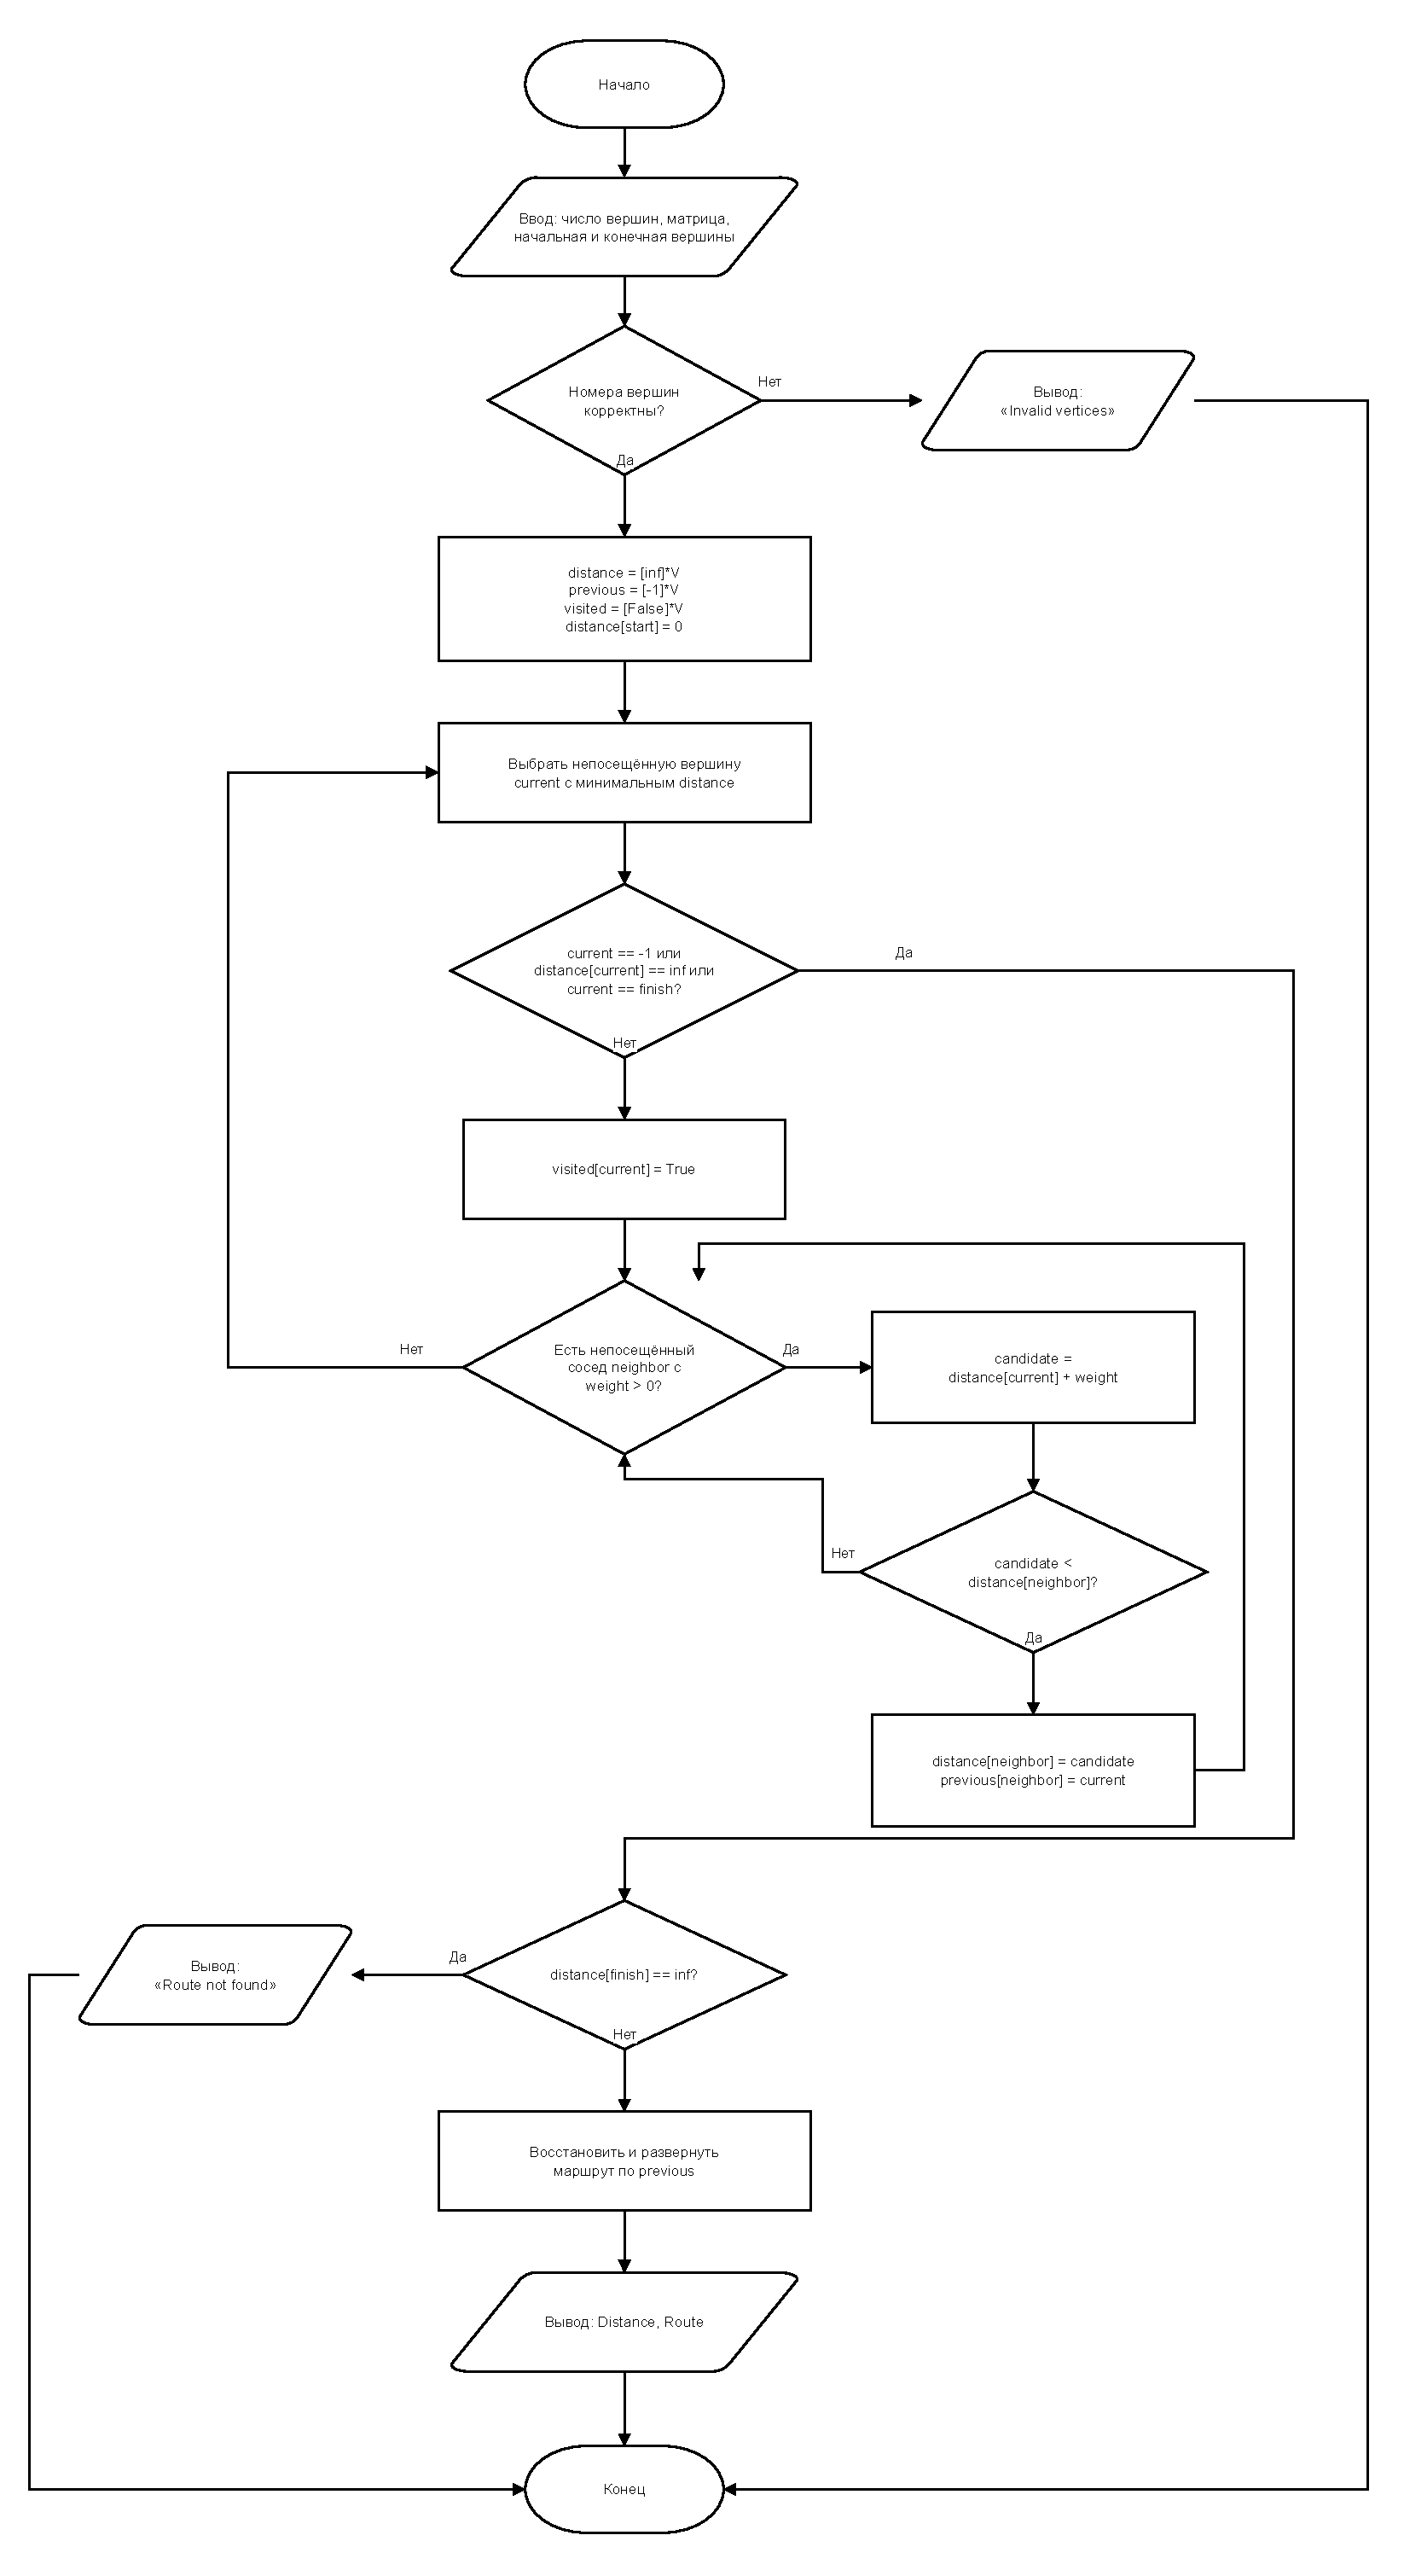
\includegraphics[width=\linewidth,height=0.86\textheight,keepaspectratio]{final-qwen-python.pdf}
  \caption{Итоговая блок-схема Python от Qwen3.7-Plus в формате draw.io}\label{fig:qwen-python}
\end{figure}

\begin{figure}[p]
  \centering
  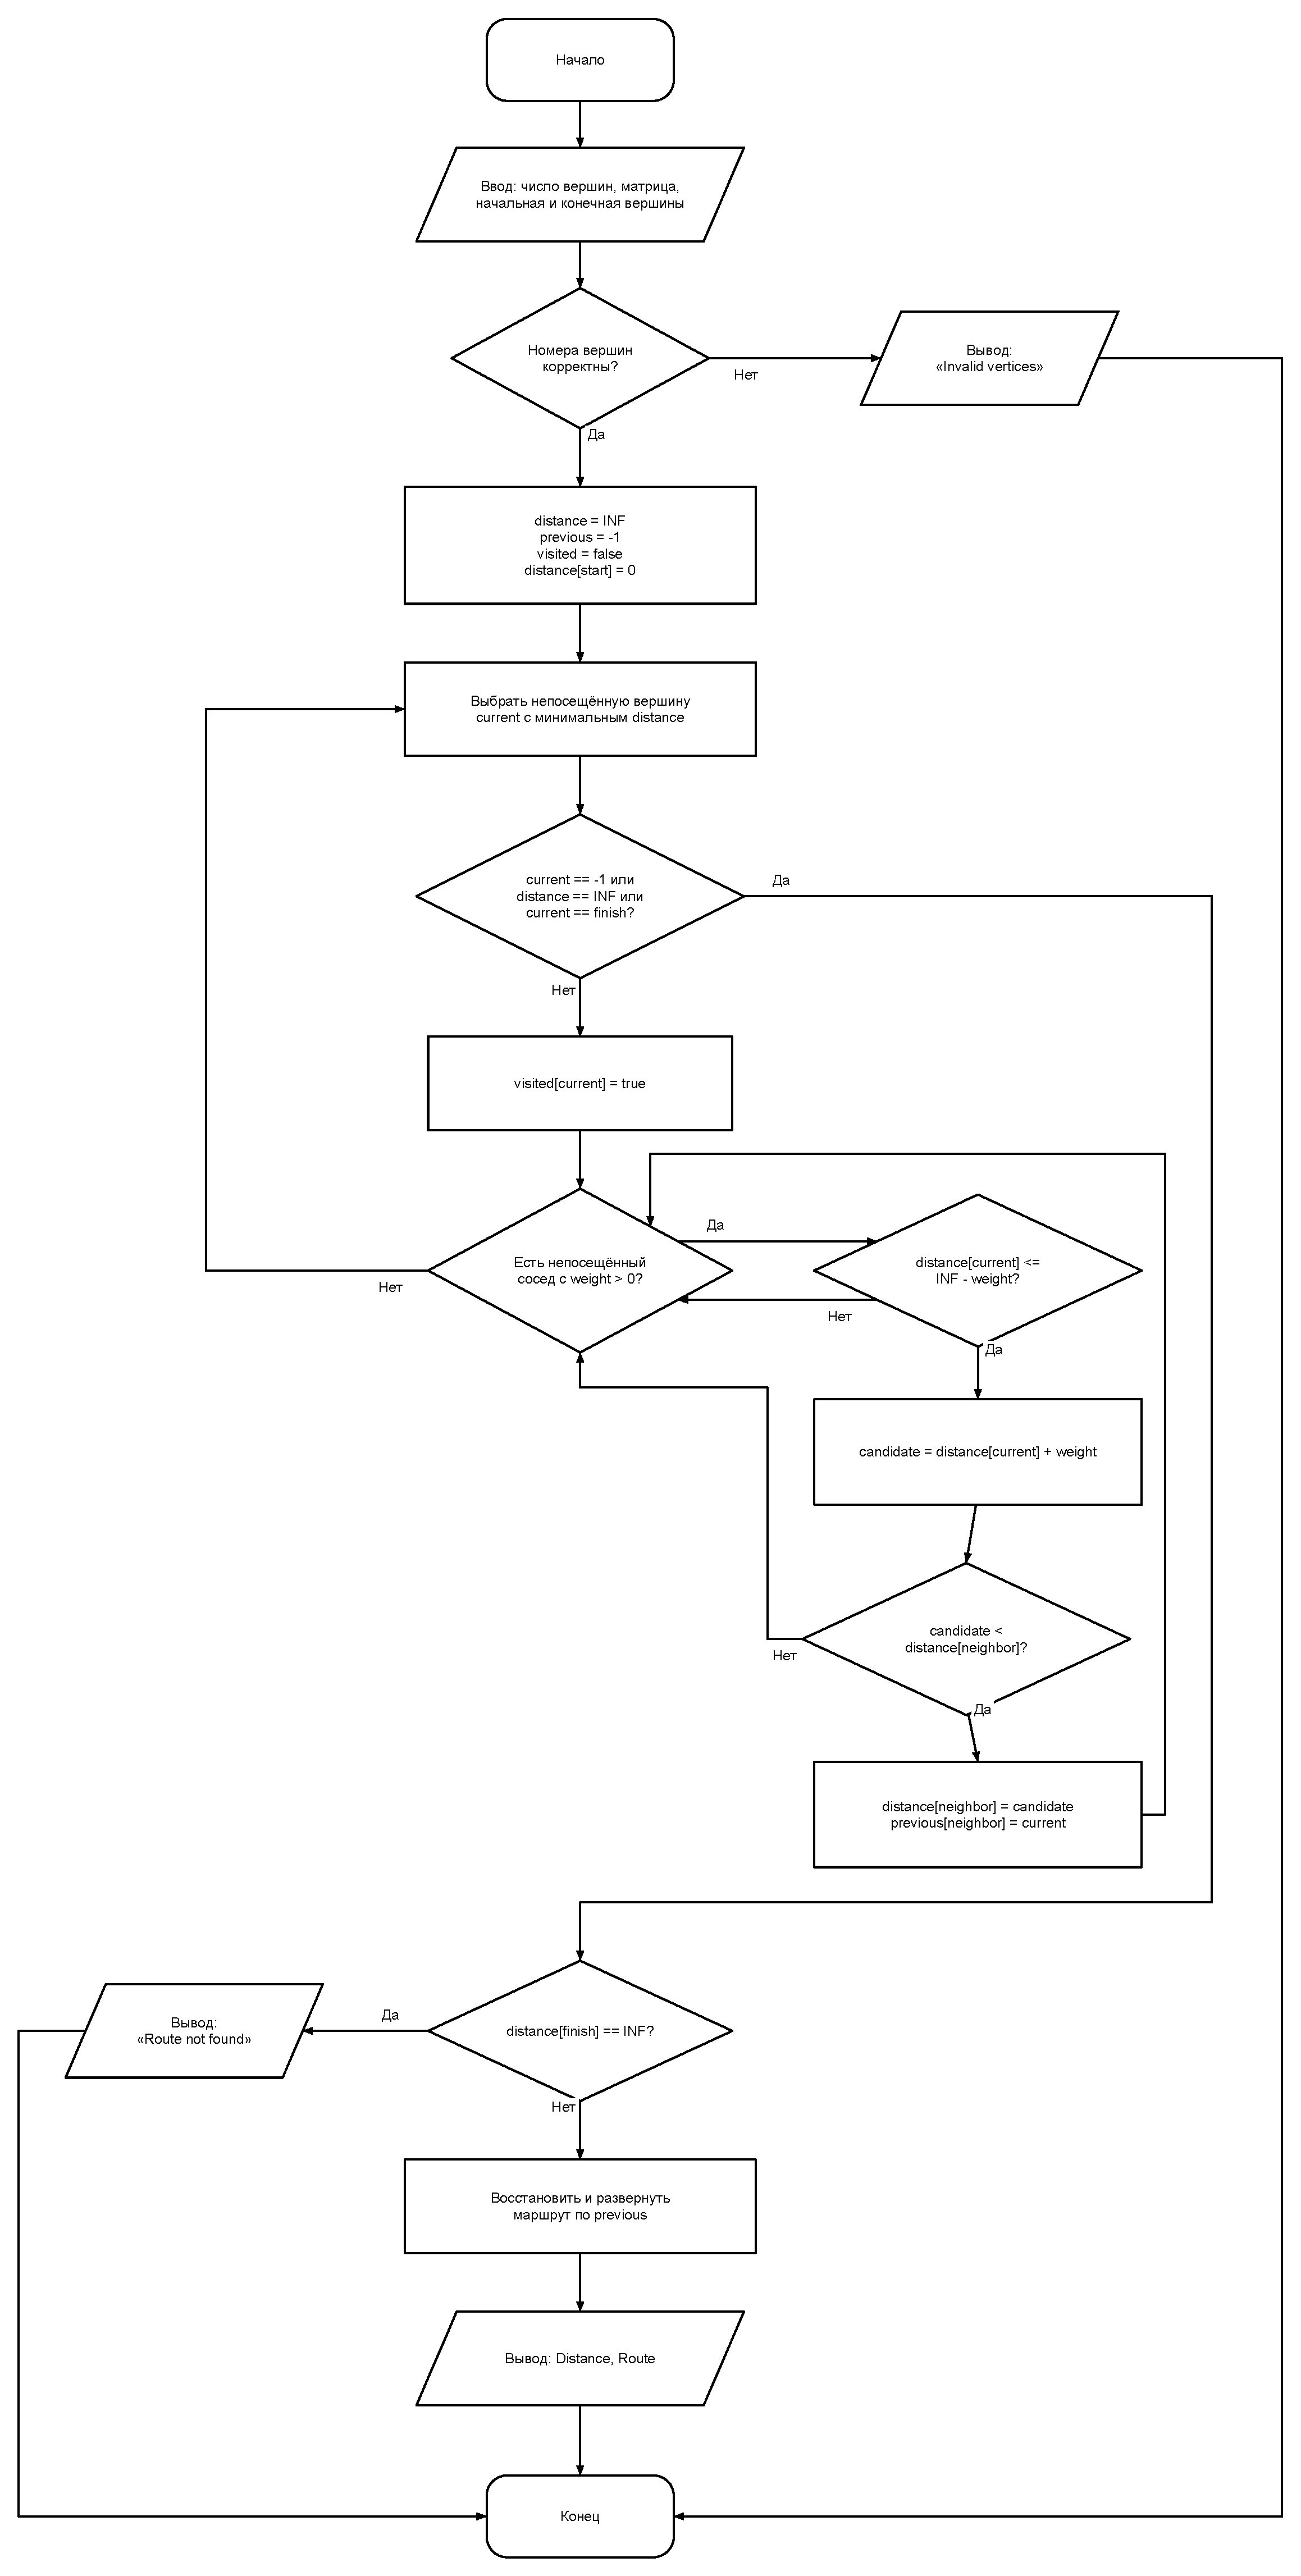
\includegraphics[width=\linewidth,height=0.86\textheight,keepaspectratio]{final-qwen-cpp.pdf}
  \caption{Итоговая блок-схема C++ от Qwen3.7-Plus в формате yEd GraphML}\label{fig:qwen-cpp}
\end{figure}

\begin{figure}[p]
  \centering
  Python (draw.io)\par\smallskip
  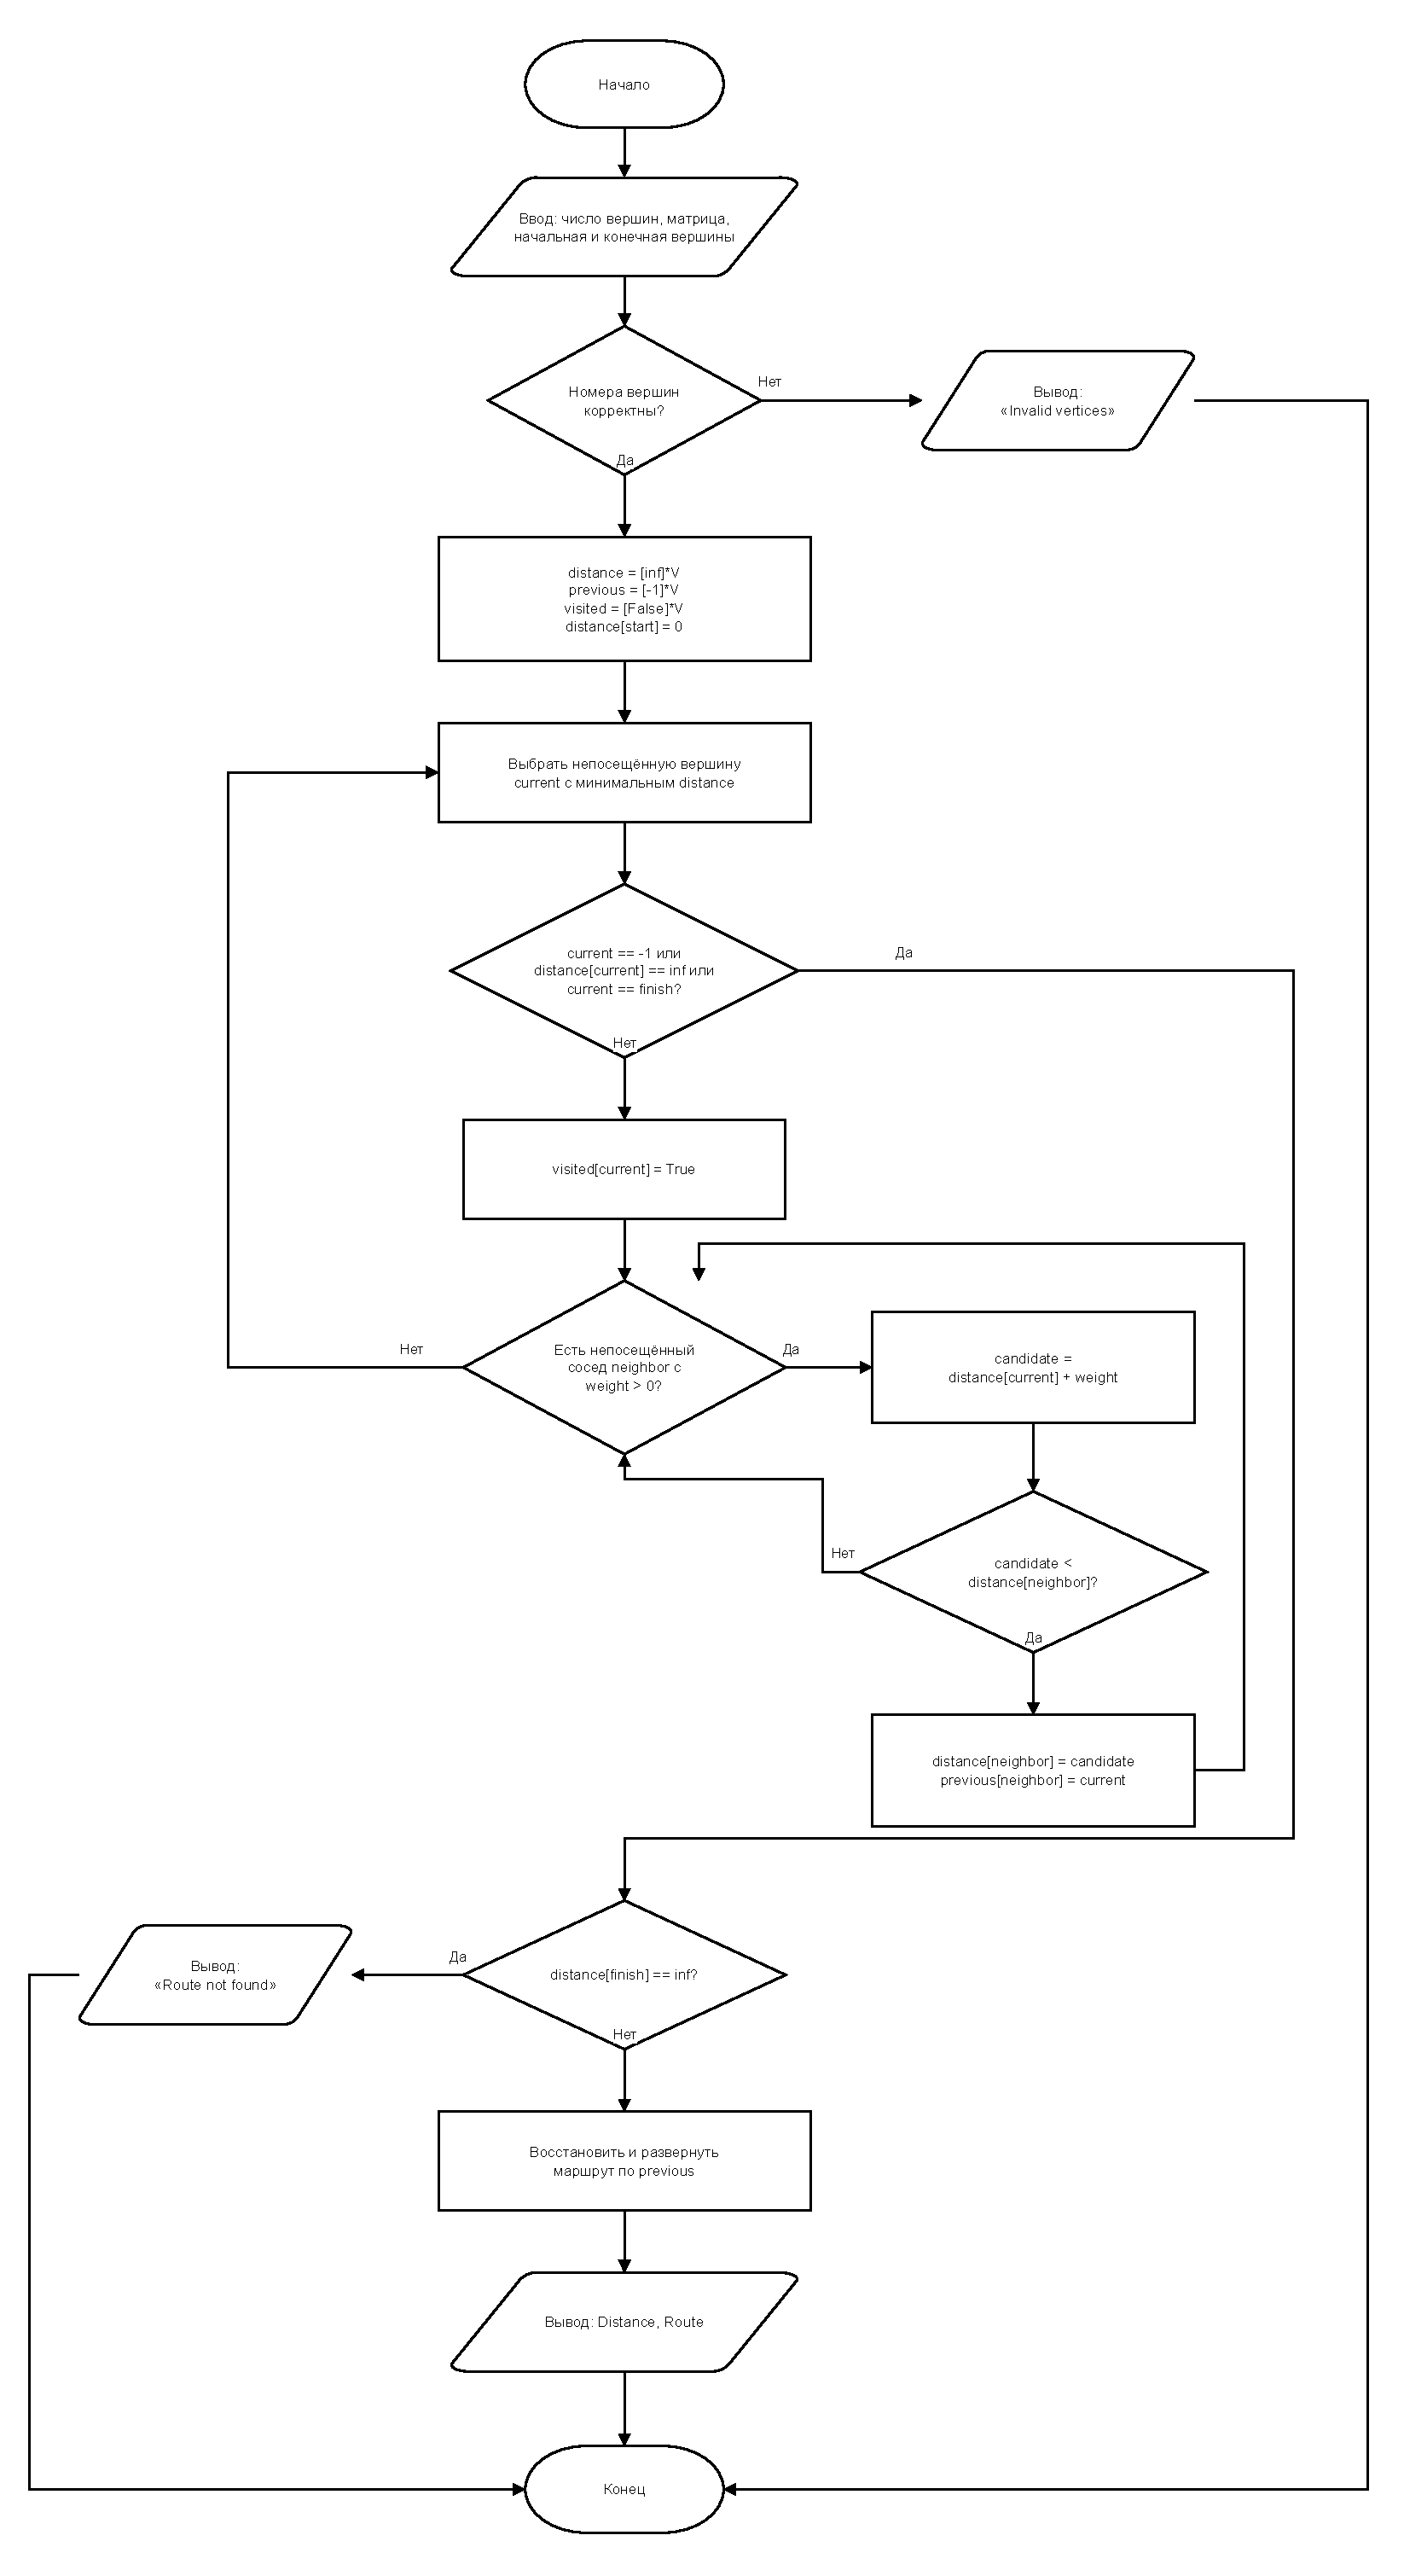
\includegraphics[viewport=245 1164.12 705 1354.12,clip,width=\linewidth,height=0.38\textheight,keepaspectratio]{final-qwen-python.pdf}
  \par\medskip
  C++ (GraphML)\par\smallskip
  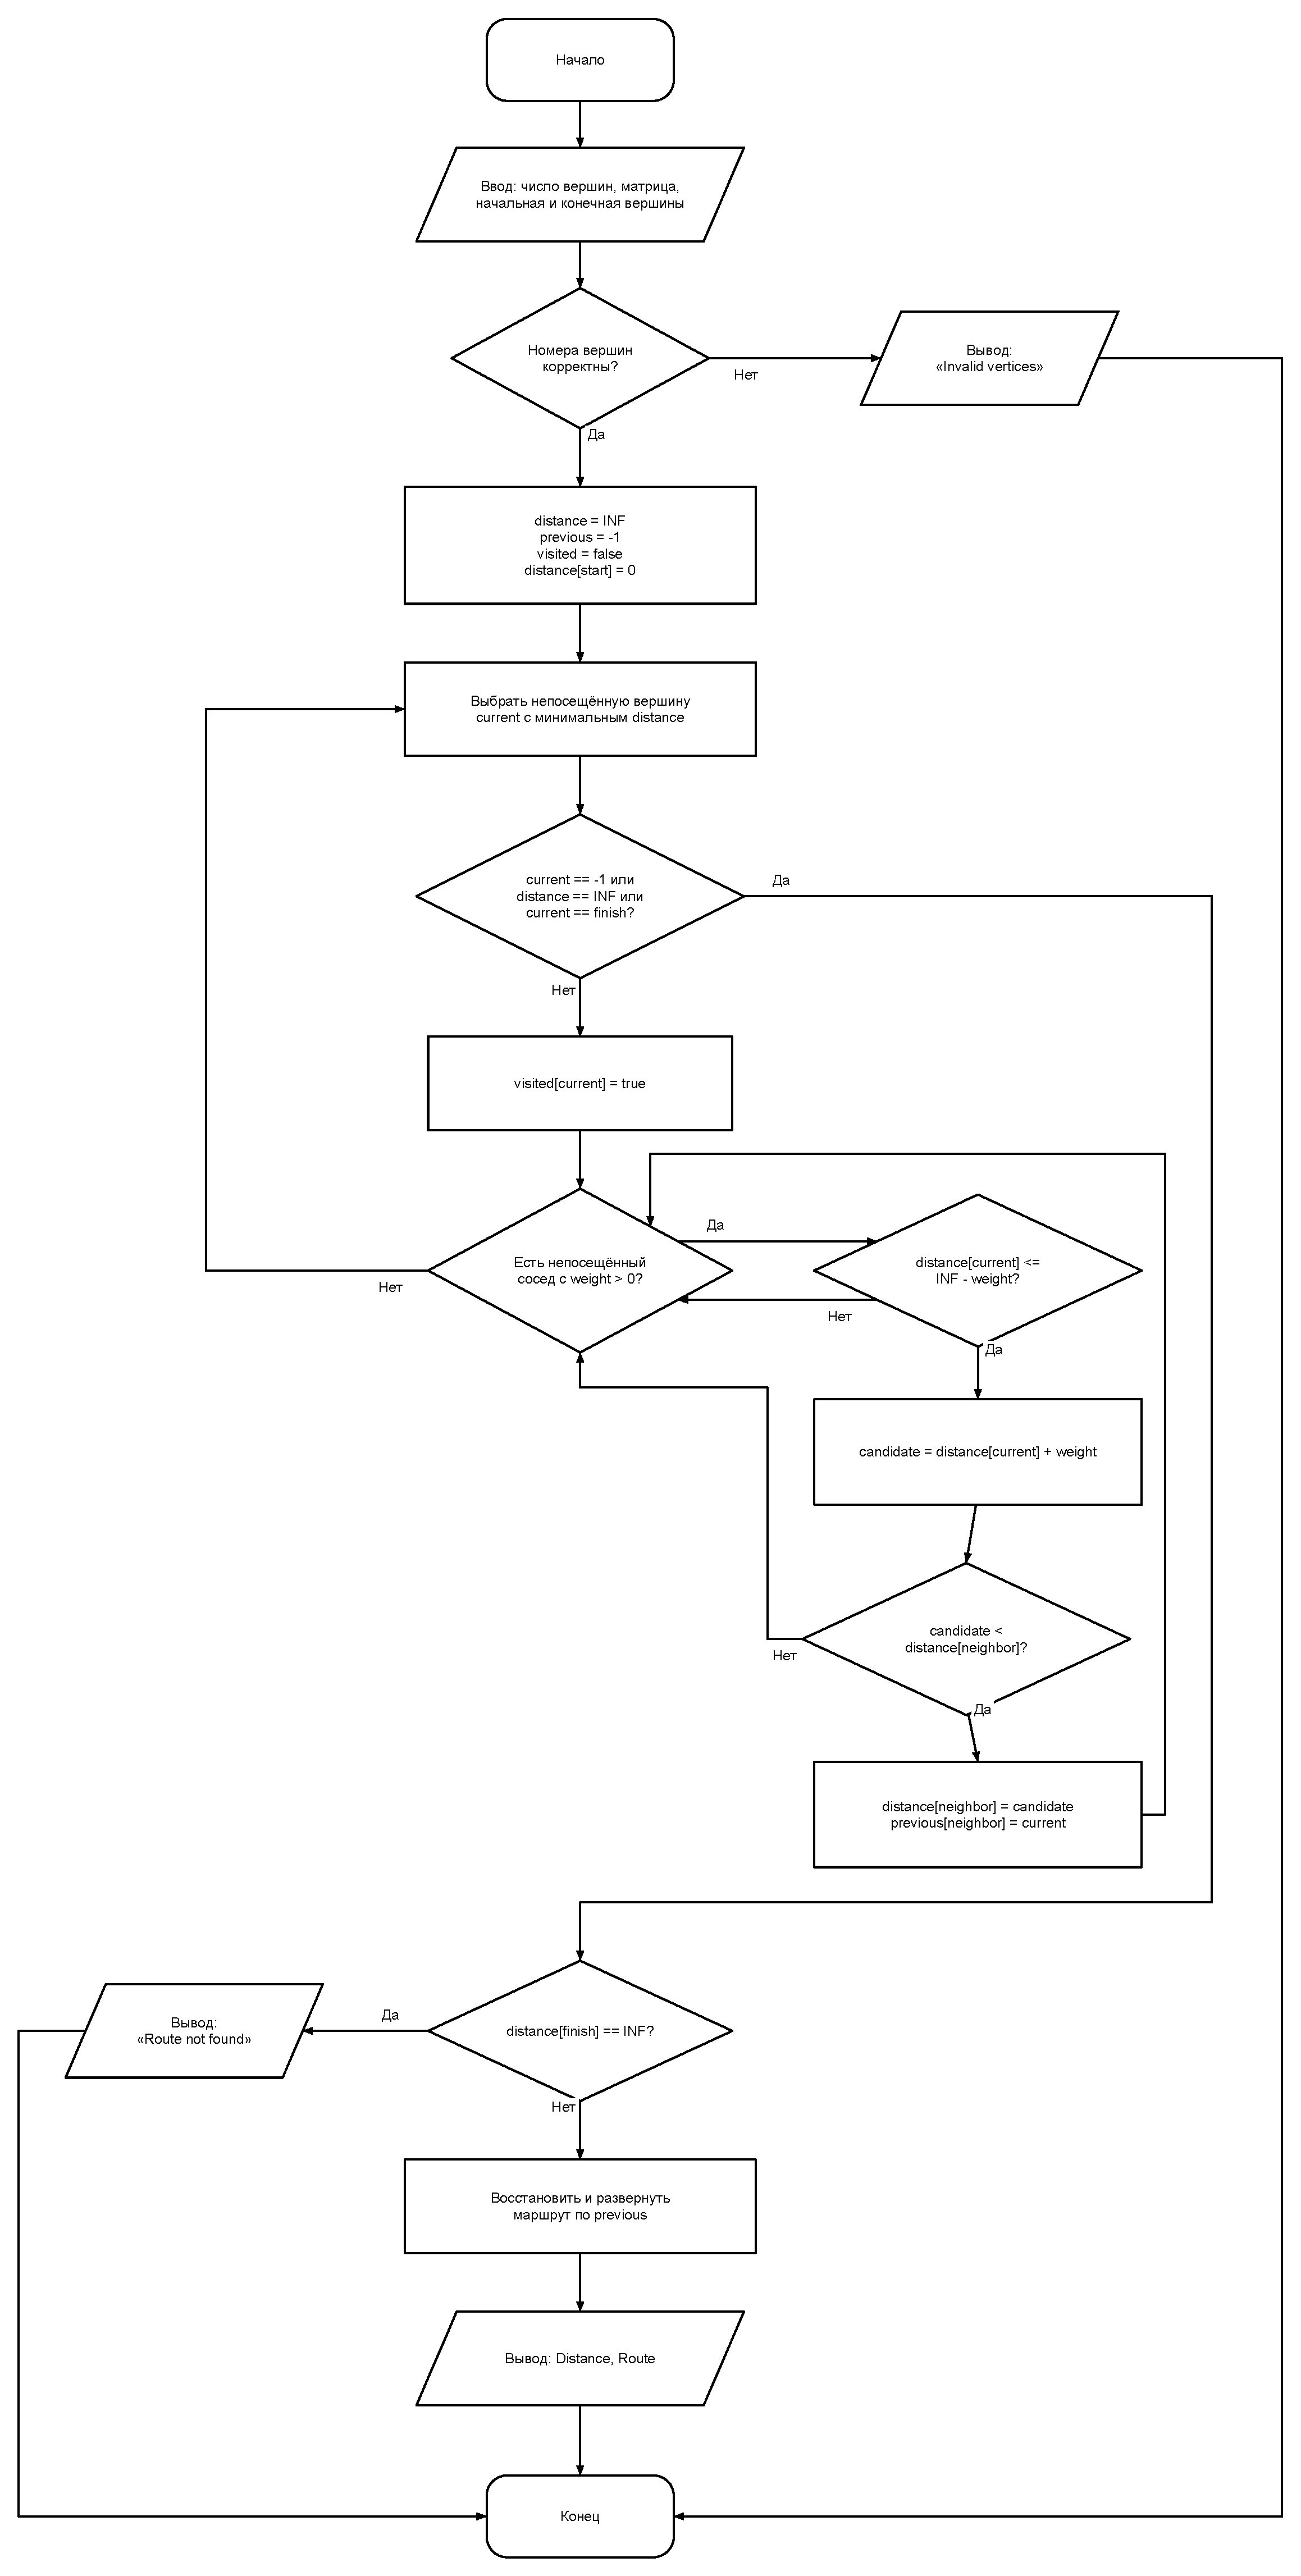
\includegraphics[viewport=340 1807 990 2092,clip,width=\linewidth,height=0.38\textheight,keepaspectratio]{final-qwen-cpp.pdf}
  \caption{Проверка входных индексов в итоговых схемах Qwen3.7-Plus}\label{fig:qwen-detail}
\end{figure}

\begin{figure}[p]
  \centering
  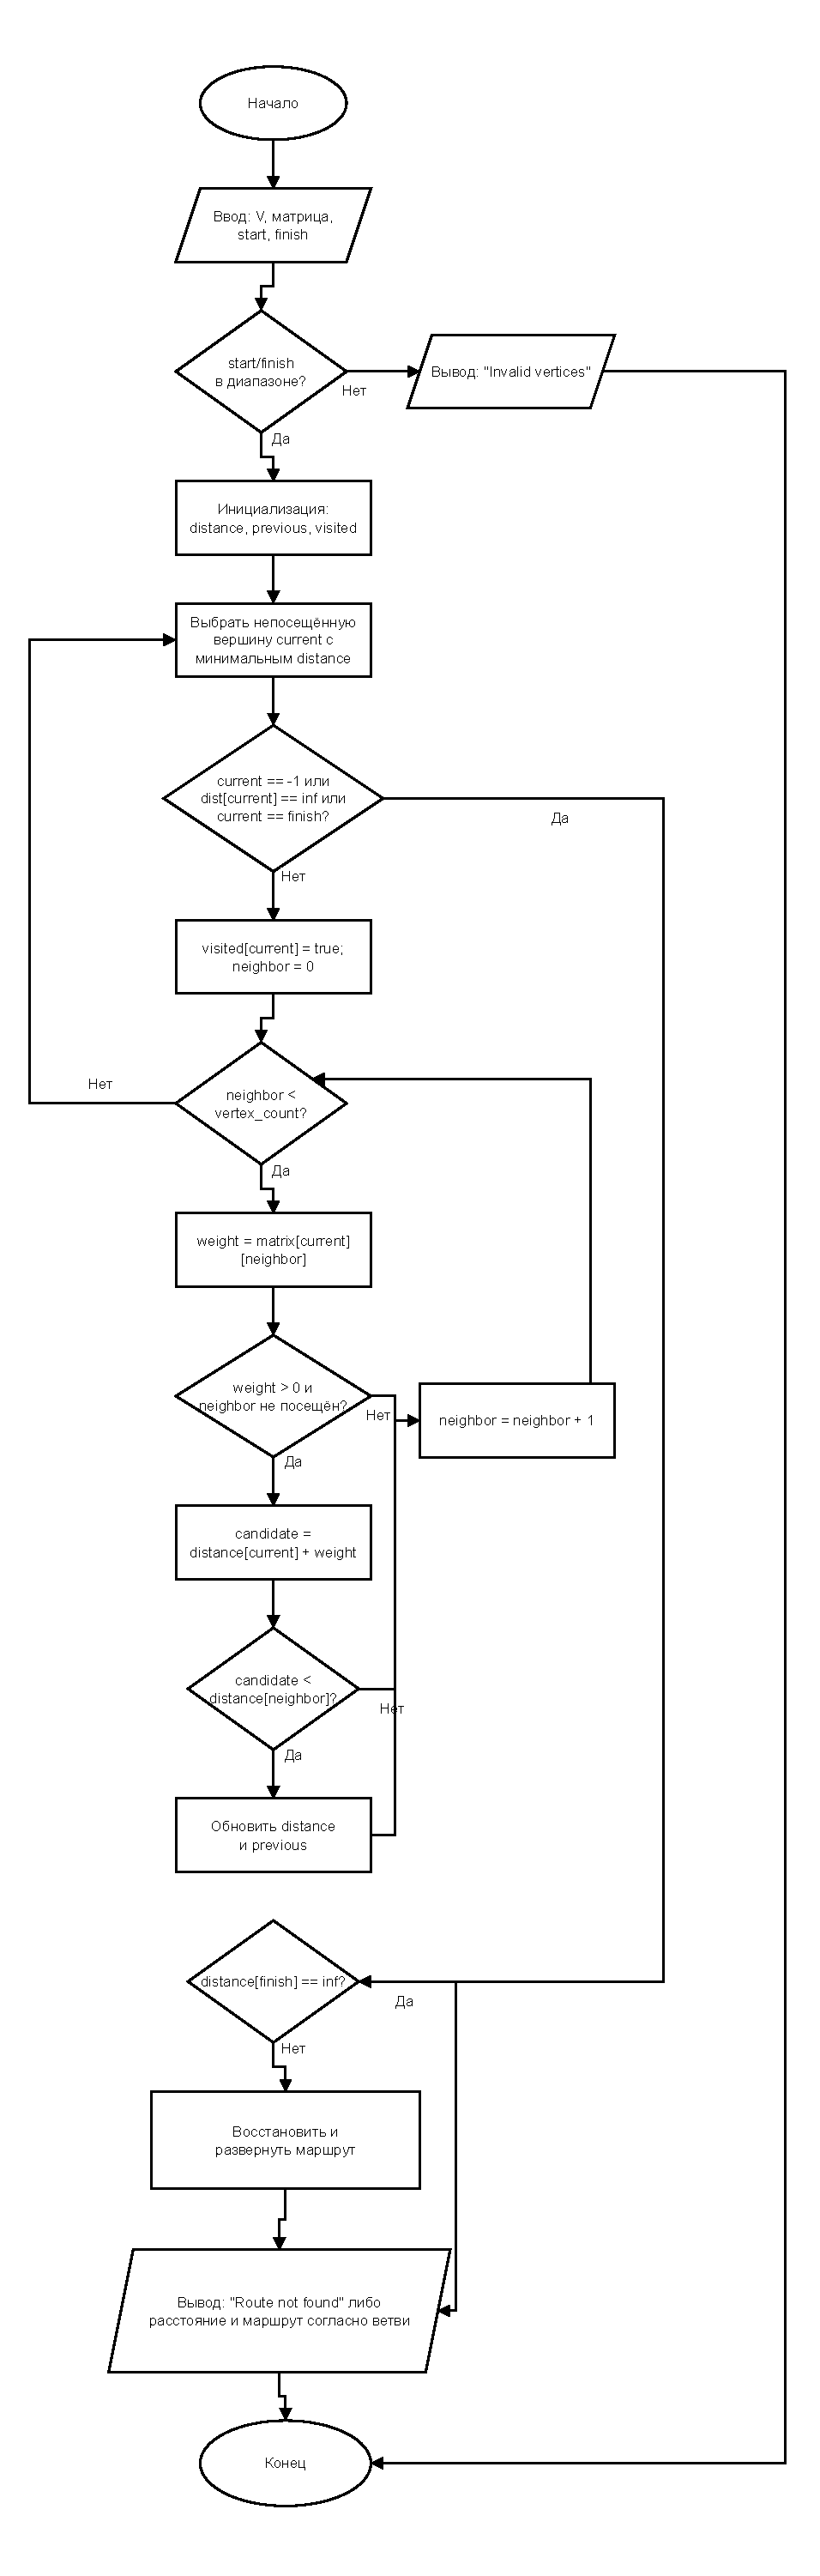
\includegraphics[width=\linewidth,height=0.86\textheight,keepaspectratio]{final-korolev-python.pdf}
  \caption{Итоговая блок-схема Python от Korolev AI в формате draw.io}\label{fig:korolev-python}
\end{figure}

\begin{figure}[p]
  \centering
  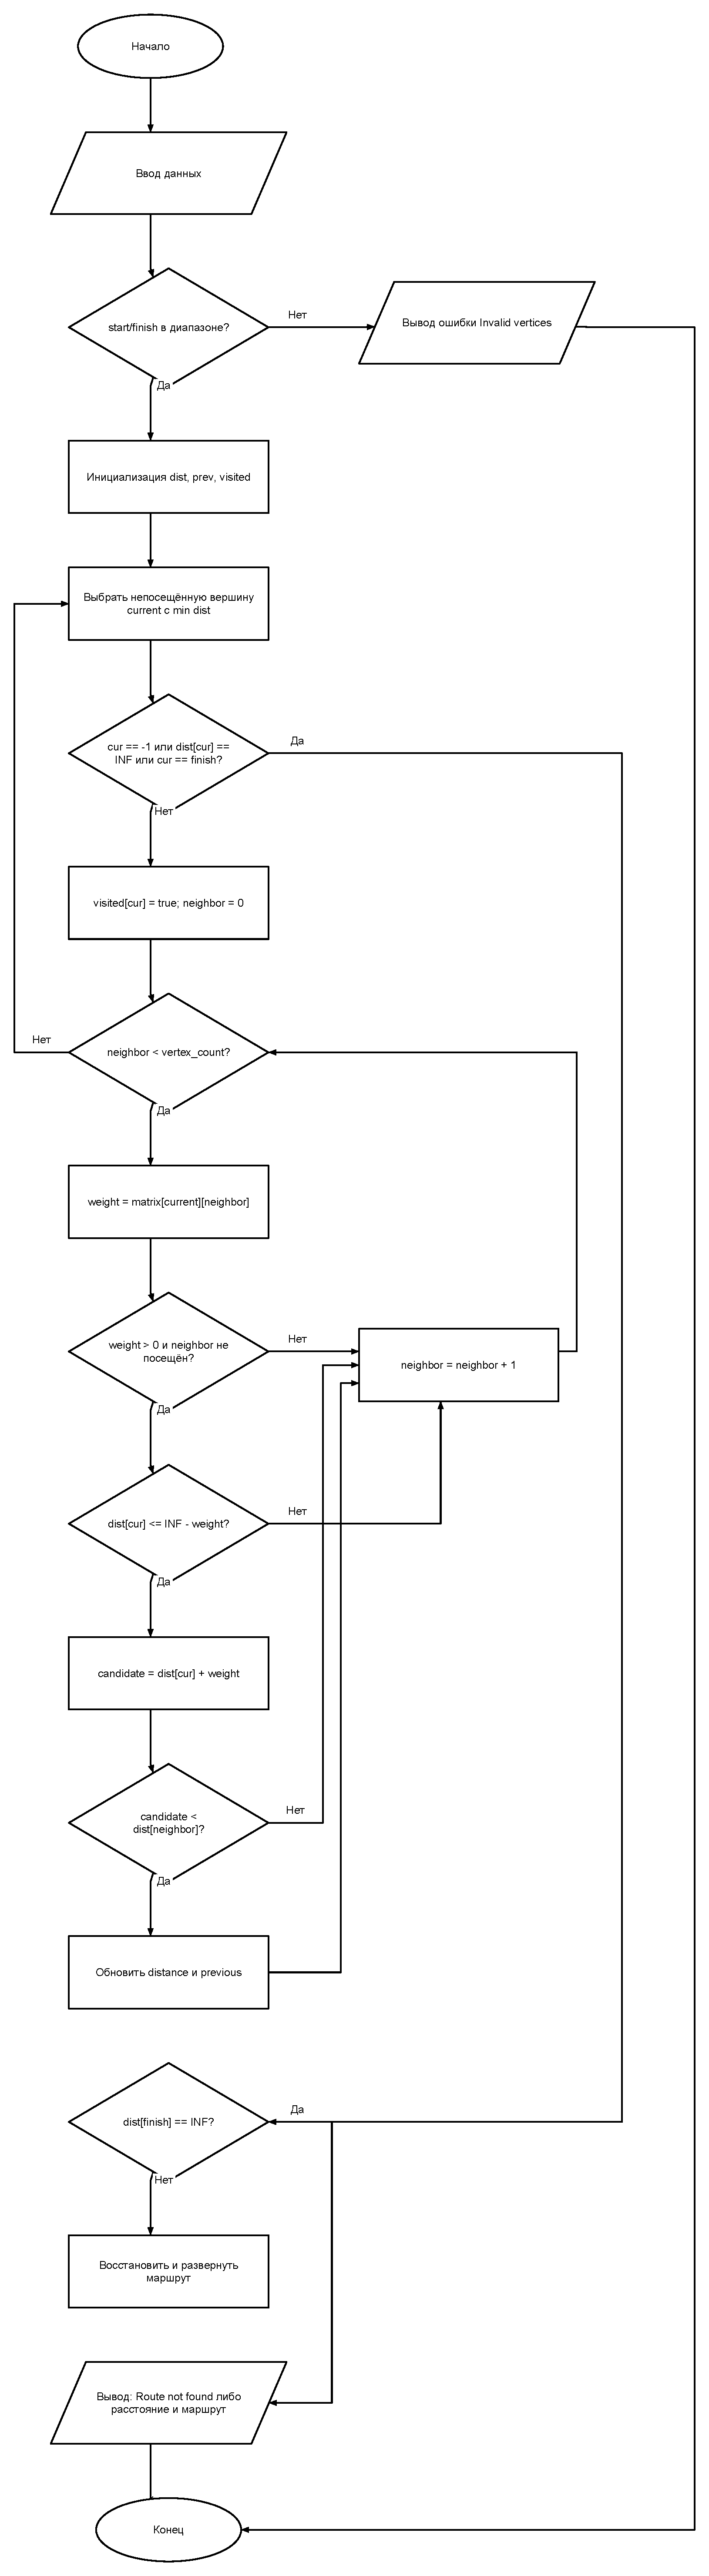
\includegraphics[width=\linewidth,height=0.86\textheight,keepaspectratio]{final-korolev-cpp.pdf}
  \caption{Итоговая блок-схема C++ от Korolev AI в формате yEd GraphML}\label{fig:korolev-cpp}
\end{figure}

\begin{figure}[p]
  \centering
  Python (draw.io)\par\smallskip
  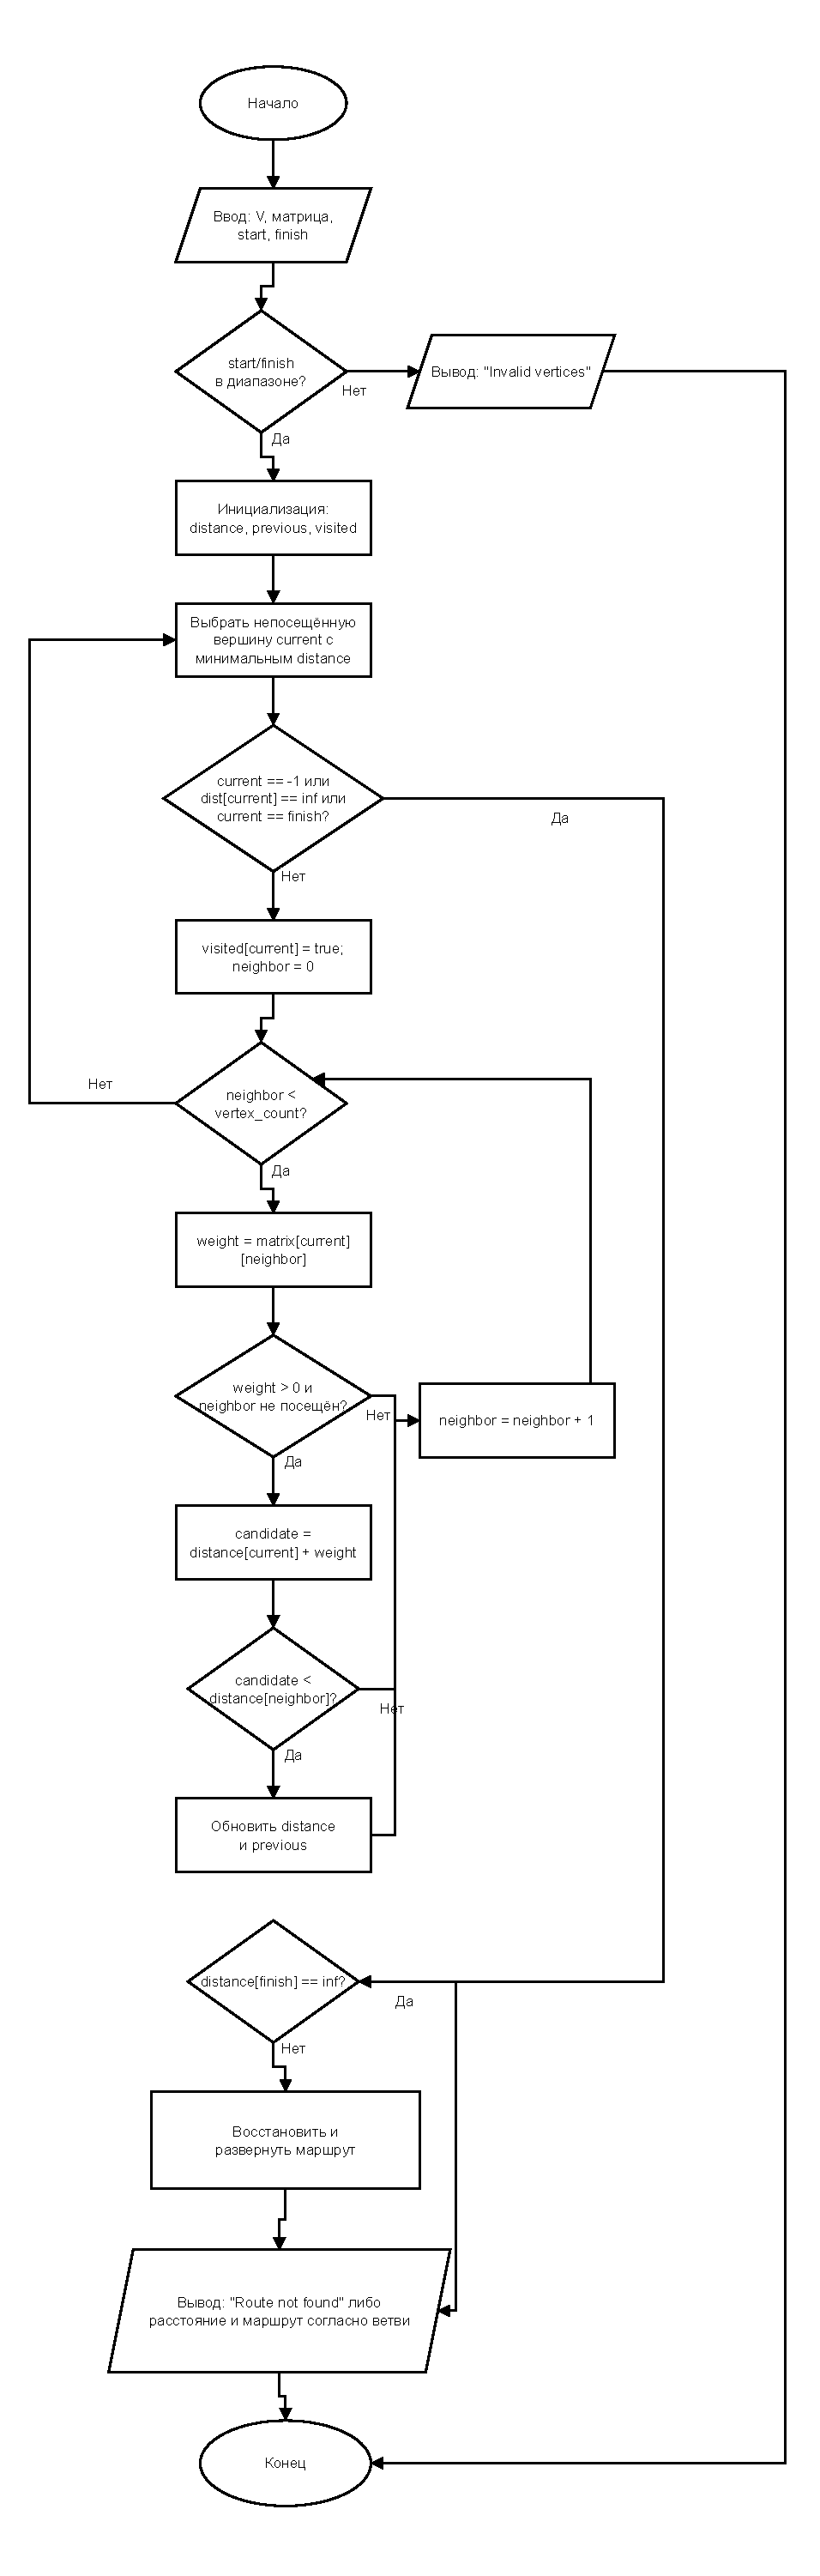
\includegraphics[viewport=84 1176.96 361 1350.96,clip,width=\linewidth,height=0.38\textheight,keepaspectratio]{final-korolev-python.pdf}
  \par\medskip
  C++ (GraphML)\par\smallskip
  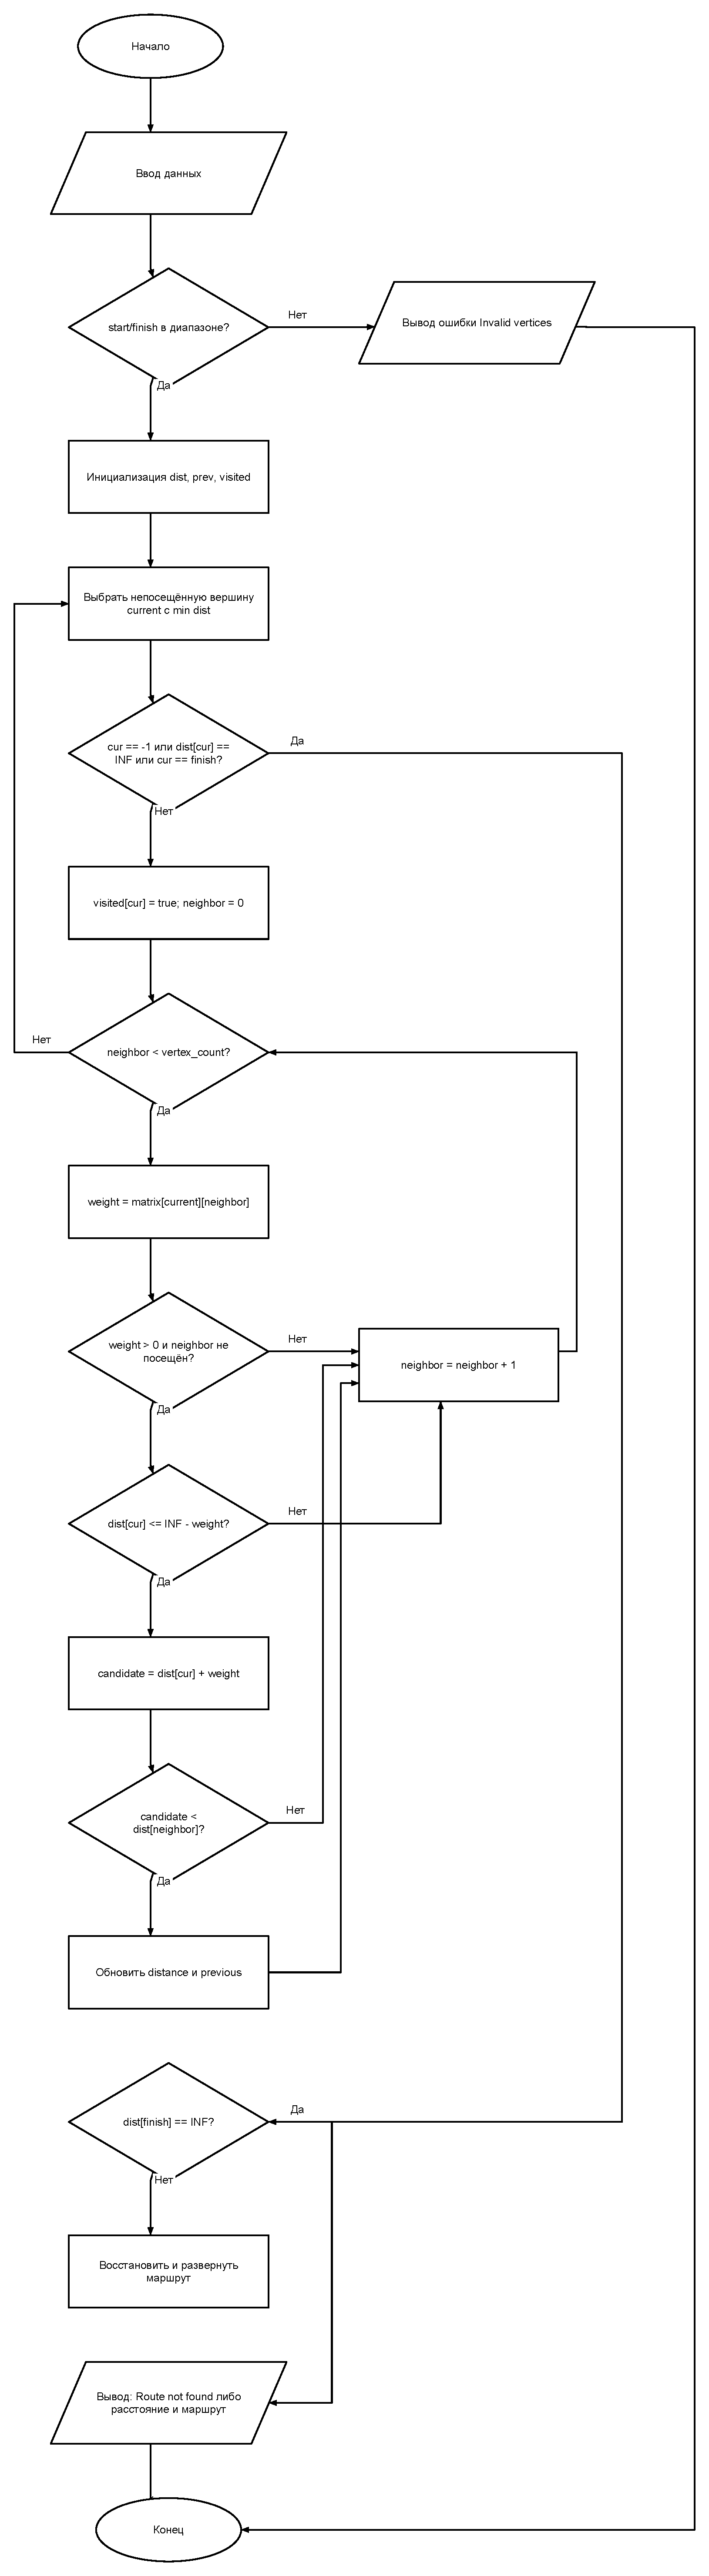
\includegraphics[viewport=43 2390 669 2713,clip,width=\linewidth,height=0.38\textheight,keepaspectratio]{final-korolev-cpp.pdf}
  \caption{Проверка входных индексов в итоговых схемах Korolev AI}\label{fig:korolev-detail}
\end{figure}

\begin{figure}[p]
  \centering
  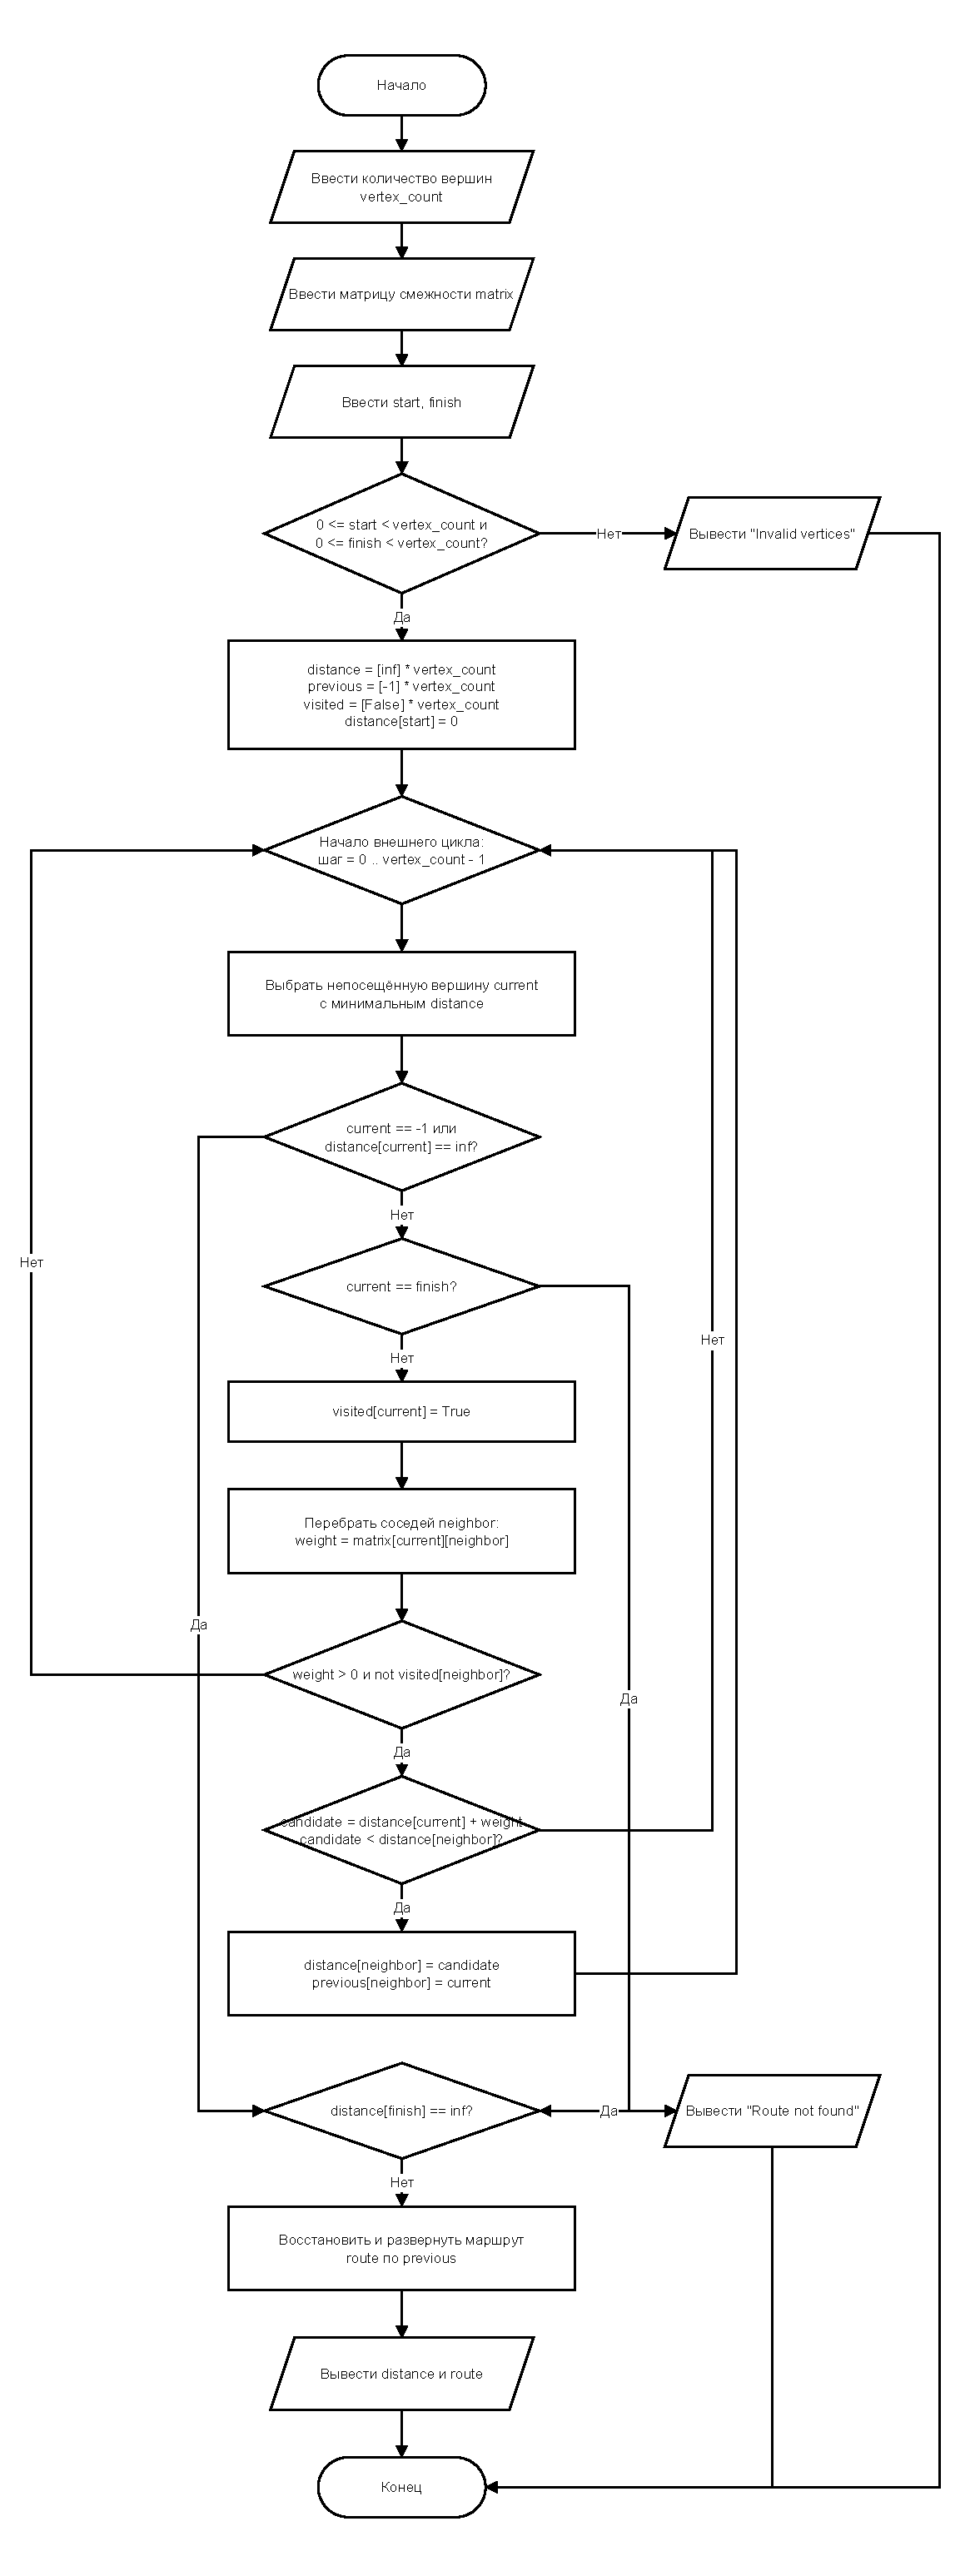
\includegraphics[width=\linewidth,height=0.86\textheight,keepaspectratio]{final-deepseek-python.pdf}
  \caption{Итоговая блок-схема Python от DeepSeek в формате draw.io}\label{fig:deepseek-python}
\end{figure}

\begin{figure}[p]
  \centering
  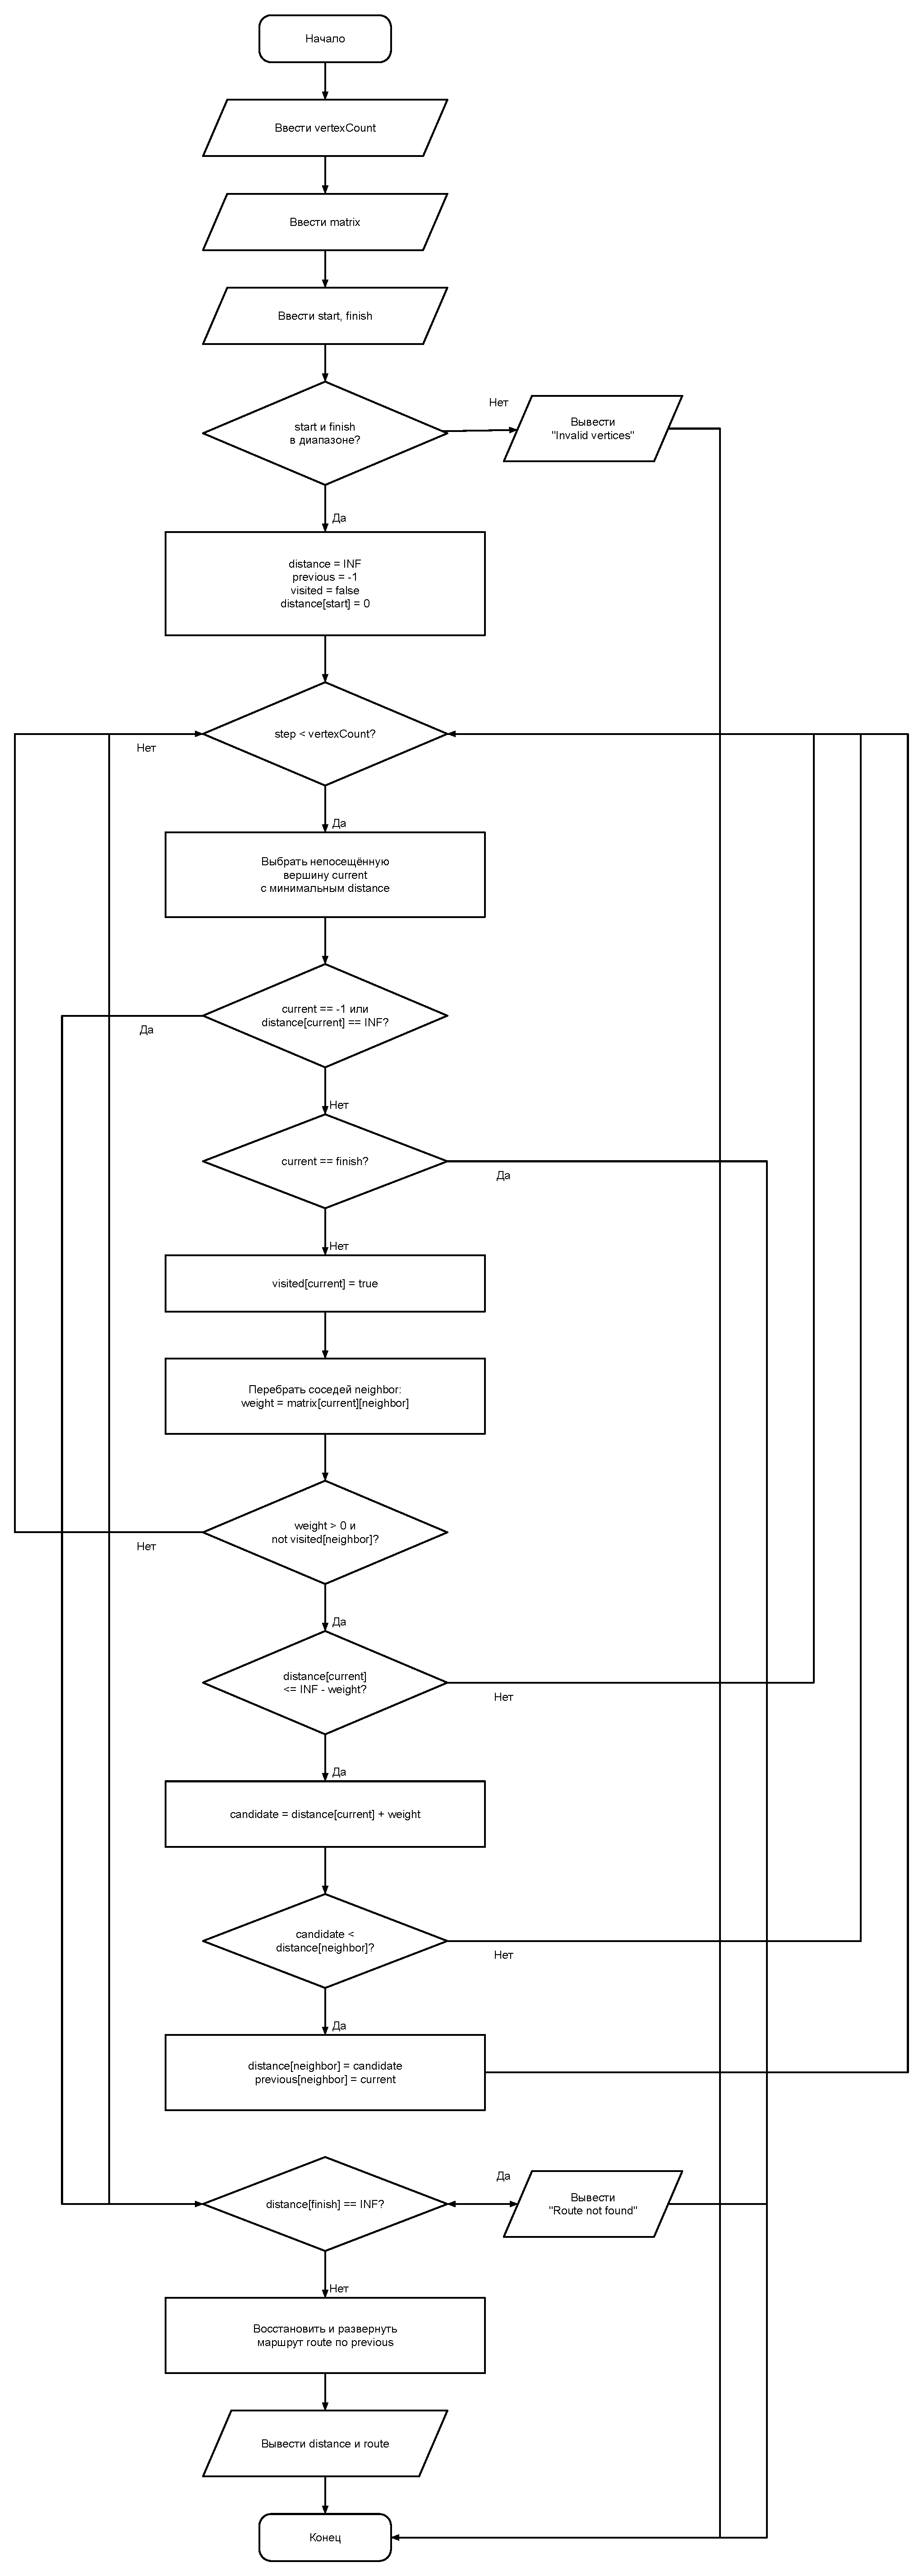
\includegraphics[width=\linewidth,height=0.86\textheight,keepaspectratio]{final-deepseek-cpp.pdf}
  \caption{Итоговая блок-схема C++ от DeepSeek в формате yEd GraphML}\label{fig:deepseek-cpp}
\end{figure}

\begin{figure}[p]
  \centering
  Python (draw.io)\par\smallskip
  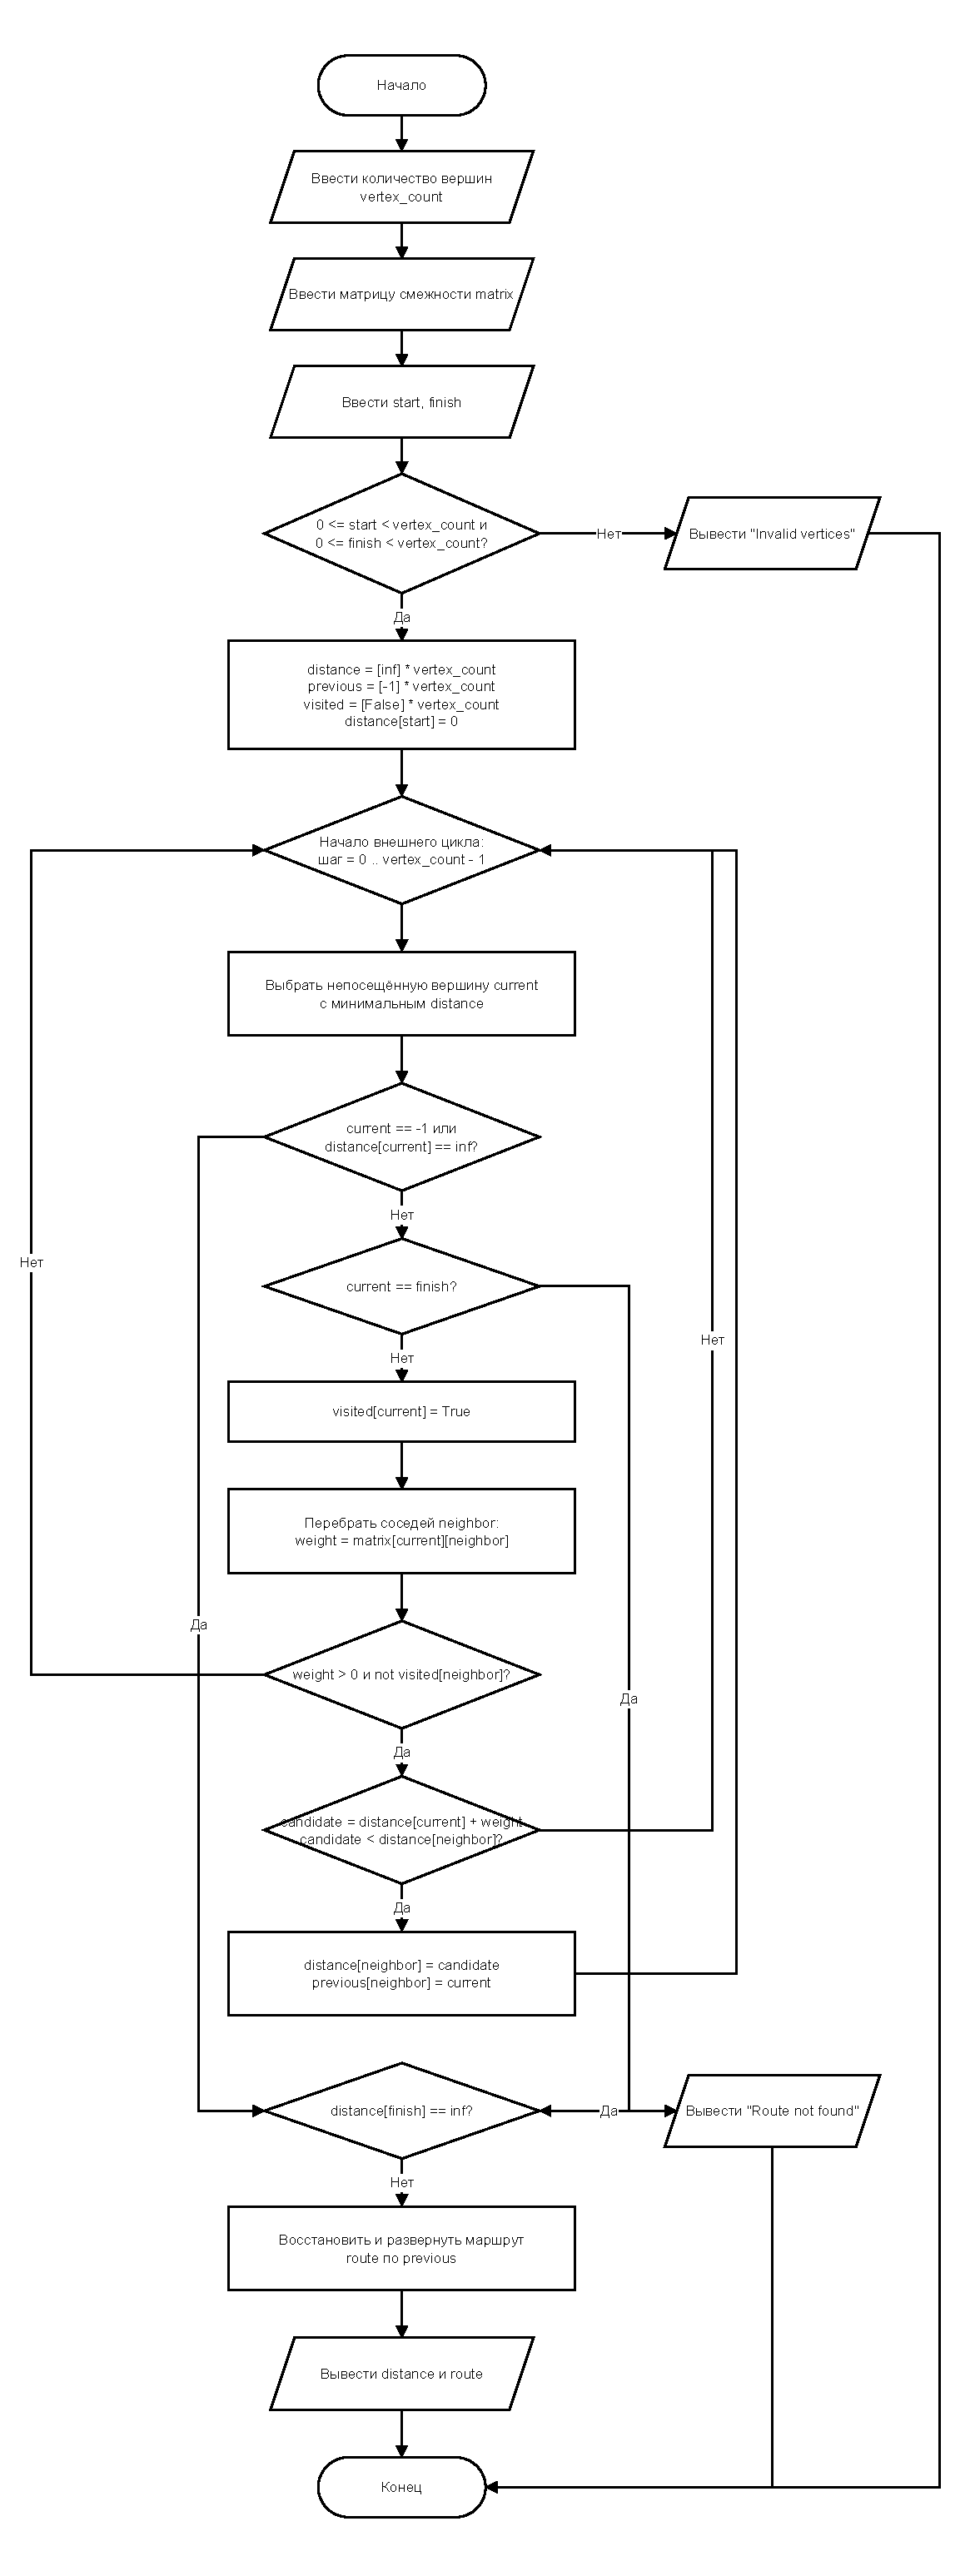
\includegraphics[viewport=145 1115.12 527 1289.12,clip,width=\linewidth,height=0.38\textheight,keepaspectratio]{final-deepseek-python.pdf}
  \par\medskip
  C++ (GraphML)\par\smallskip
  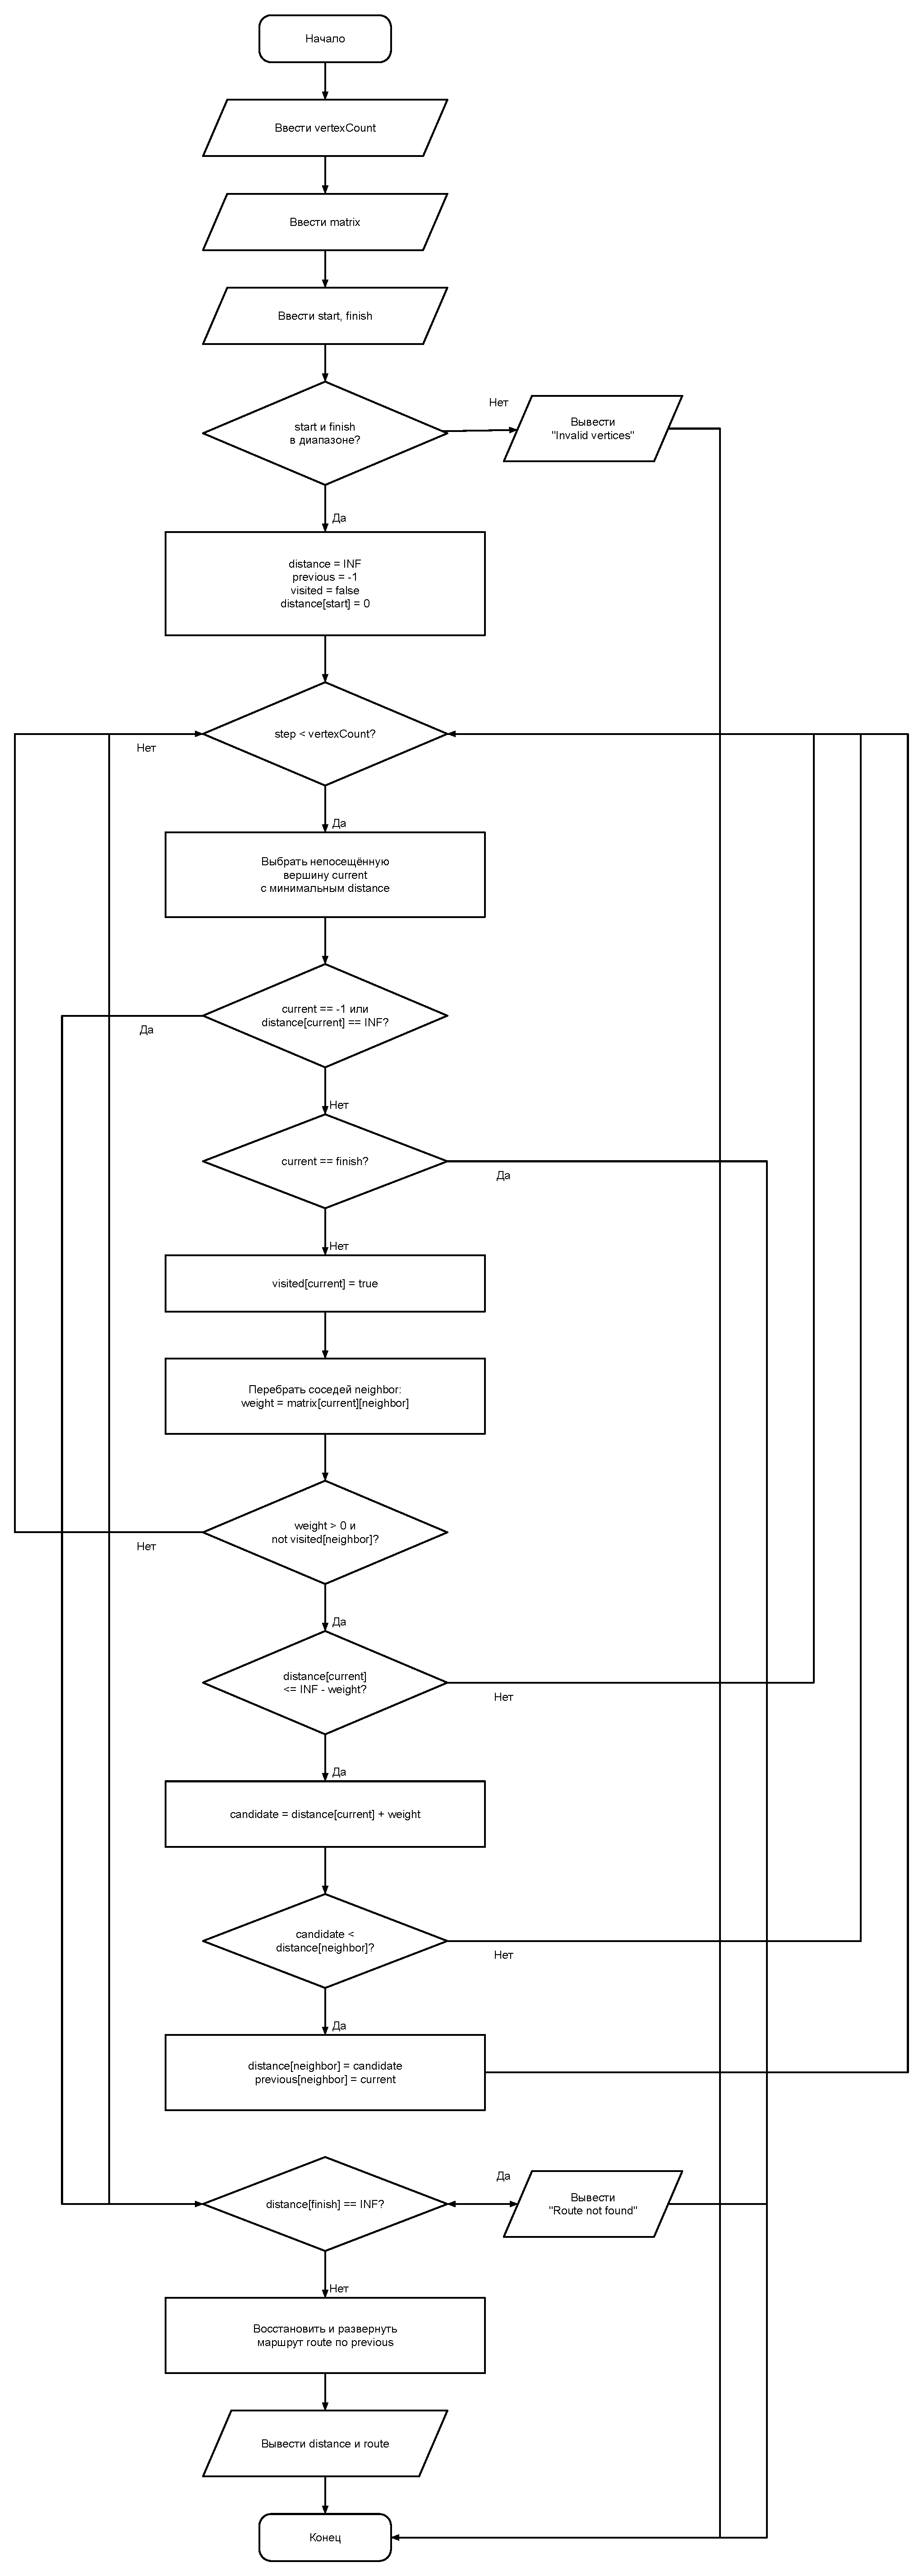
\includegraphics[viewport=200 2182 745 2452,clip,width=\linewidth,height=0.38\textheight,keepaspectratio]{final-deepseek-cpp.pdf}
  \caption{Проверка входных индексов в итоговых схемах DeepSeek}\label{fig:deepseek-detail}
\end{figure}
\clearpage

\section{Выводы по исследовательскому разделу}

Синтаксическая корректность XML оказалась необходимым, но недостаточным условием. Наиболее показателен Qwen: две версии прошли автоматический контроль и были отклонены после открытия. XML-анализ подтверждал существование путей, но не оценивал читаемость общей композиции.

DeepSeek показал наиболее короткую цепочку. Qwen точнее воспроизводил поздние локальные изменения, но плохо планировал схему целиком. Korolev AI показал наименьшую устойчивость и максимальную стоимость ручного сопровождения.

Первый содержательный вывод состоит в том, что генерацию блок-схем следует рассматривать как задачу с двумя независимыми уровнями качества. Первый уровень --- машинная корректность файла, второй --- коммуникативная пригодность визуального представления. Проверка только одного уровня приводит либо к принятию нечитаемого документа, либо к субъективной оценке без контроля структуры.

Второй вывод связан с формой обратной связи. Общие указания эффективны только на ранних шагах, когда требуется исправить очевидный класс ошибок. Для сложных схем необходимо переходить к проверяемым ограничениям: идентификаторам элементов, сторонам портов, допустимым областям и координатным коридорам. Одновременно следует ограничивать область изменений, иначе исправление одного дефекта может породить несколько новых.

Третий вывод касается момента отказа от локальных правок. Если независимые рёбра уже используют общие коридоры и взаимосвязи не прослеживаются, последовательные малые смещения способны лишь усложнить схему. В такой ситуации полная перекомпоновка по заранее определённой архитектуре оказывается эффективнее, что подтвердил поздний этап работы с Qwen.

Наконец, итоговая диаграмма не позволяет сама по себе оценить вклад модели. Аккуратный файл может быть результатом длинной серии уточнений, ручного задания геометрии и восстановления регрессий. Поэтому при сравнении БЯМ необходимо сохранять протокол взаимодействия, а не только конечный артефакт.

\section{Стабильность исправлений и ограничения исследования}

\subsection{Методика анализа стабильности}

Стабильность понималась как сохранение уже корректных элементов при следующем ответе. После каждой правки повторно проверялся весь файл. Эта методика выявила удаления операторов, новые пересечения и ухудшения компоновки, не связанные напрямую с заданным исправлением.

Для анализа стабильности сравнивались не только визуальные изображения, но и исходные XML. Проверялось, какие узлы, рёбра, подписи и координаты изменились между соседними версиями. Если корректирующий запрос относился к одному ребру, а модель переписывала несколько независимых узлов, такая версия считалась потенциально нестабильной даже при отсутствии немедленно заметной ошибки.

Наиболее опасны смысловые регрессии, поскольку они могут быть малозаметны на общей схеме. Удаление оператора равенства или изменение текста условия внешне не нарушает геометрию, но меняет интерпретацию алгоритма. Поэтому повторная проверка полного текста блоков обязательна даже после чисто пространственного запроса.

\subsection{Роль визуальной проверки}

Редакторы интерпретируют геометрию, порты и модели подписей сложнее простого XML-анализатора. Поэтому окончательное принятие выполнялось пользователем после открытия файлов. Автоматический PASS не трактовался как подтверждение визуального качества.

Ручная проверка выполняет роль интеграционного теста: она проверяет совместную работу XML-структуры и конкретного механизма визуализации. Особенно важны переносы строк и внутренние области подписи, поскольку фактическая ширина текста зависит от шрифта и параметров редактора. Также визуально обнаруживаются слияние близких линий, двусмысленность меток и слишком длинные маршруты, формально не пересекающие ни одного узла.

При этом ручная оценка не отменяет автоматический анализ. Человек может не заметить отсутствующую ссылку, дублирующий идентификатор или изменение скрытого атрибута, особенно в большой схеме. Надёжность обеспечивается последовательностью двух методов: сначала автоматический контроль допускает файл к просмотру, затем визуальная проверка оценивает его как средство представления алгоритма.

\subsection{Границы применимости результатов}

Не выполнялись независимые повторные генерации и формальная экспертная оценка эстетики. Исследована одна задача и одна цепочка на сервис. Результаты документируют наблюдаемый процесс, но не устанавливают статистическое превосходство одной модели для всех типов диаграмм.

Дополнительным ограничением является неодинаковая внутренняя сложность финальных схем: модели могли по-разному детализировать внутренний цикл, сохраняя эквивалентную логику. Количество элементов поэтому использовалось для описания результата, но не как самостоятельный показатель качества. Также не сравнивались стоимость доступа к сервисам, энергопотребление и аппаратная производительность их серверов.

Для повышения обобщаемости следовало бы выполнить несколько независимых запусков каждой модели, изменить тип алгоритма и привлечь нескольких экспертов с заранее определённой шкалой читаемости. Полезно также измерять фактическое время генерации, время ручной проверки и объём корректирующих запросов. В настоящей работе эти направления рассматриваются как продолжение исследования, а выводы ограничиваются зафиксированными цепочками.

\chapter*{ЗАКЛЮЧЕНИЕ}
\addcontentsline{toc}{chapter}{ЗАКЛЮЧЕНИЕ}

В работе исследована способность Qwen3.7-Plus, Korolev AI и DeepSeek создавать редактируемые блок-схемы алгоритма Дейкстры по исходным программам на Python и C++. Для каждой модели требовалось получить два различных по внутреннему устройству документа: XML draw.io и GraphML редактора yEd. В результате сформированы шесть принятых файлов, а все промежуточные ответы, проверки и корректирующие запросы сохранены как последовательный протокол эксперимента.

Поставленная цель достигнута: модели сопоставлены не по единичному демонстрационному ответу, а по полному процессу доведения результата до пригодного состояния. Такой подход позволил отделить способность сформировать синтаксически допустимый XML от способности самостоятельно спроектировать понятную диаграмму. Во всех трёх случаях первоначальная машинная корректность не гарантировала отсутствия геометрических и типографических дефектов.

Главным источником сложности стало пространственное представление управляющего потока. Основные этапы алгоритма --- инициализация, выбор вершины, релаксация, проверка достижимости и восстановление маршрута --- модели в целом распознавали правильно. Большинство дополнительных итераций потребовалось для центрирования текста, выбора корректных фигур, размещения портов, разведения длинных возвратов и устранения визуального слияния независимых рёбер. Следовательно, в исследованной задаче БЯМ лучше справлялись с логической реконструкцией алгоритма, чем с компоновкой инженерного документа.

Наиболее короткую цепочку показал DeepSeek: оба файла были приняты после шести ответов. Его преимущество связано с относительно удачной исходной draw.io-компоновкой и более устойчивыми локальными изменениями после разделения форматов. При этом результат нельзя считать полностью автоматическим: GraphML потребовал явных областей подписей, ручного размещения меток ветвей и отдельных коридоров для обратных связей. DeepSeek следует признать наиболее эффективной из трёх моделей в рамках данного эксперимента, но не инструментом, устраняющим необходимость проверки.

Qwen3.7-Plus потребовал одиннадцать ответов и занял промежуточное положение по числу итераций. Две версии прошли автоматические проверки, но были отклонены после открытия в редакторах: сначала из-за выхода текста, неверных фигур и неполных визуальных путей, затем из-за слияния рёбер и неоднозначности взаимосвязей. Приемлемый результат появился только после полной перекомпоновки по заданной координатной архитектуре и нескольких точечных исправлений. Поэтому Qwen нельзя охарактеризовать как модель с высоким качеством самостоятельной отрисовки. Его сильная сторона проявилась позднее --- в достаточно точном выполнении детальной XML-спецификации.

Korolev AI потребовал пятнадцать итераций и показал наибольшую стоимость сопровождения. Для него были характерны регрессии вне области запрошенного изменения: исправление геометрии сопровождалось повреждением текста или логических операторов. Дополнительные трудности создали обрыв совмещённого ответа и переполнение контекста старого диалога. Несмотря на получение двух принятых файлов, модель показала наименьшую устойчивость, а завершение работы потребовало разделения форматов, новых диалогов и точного кодирования отдельных символов в XML.

Количественное сравнение --- 6, 11 и 15 ответов --- отражает число циклов генерации и проверки, но не является универсальным рейтингом моделей. Исследована одна задача и одна последовательность взаимодействия с каждым сервисом; время всех ответов систематически не измерялось. Тем не менее различия в характере ошибок позволяют сделать содержательный вывод: практическая эффективность определяется не только качеством первой версии, но и локальностью исправлений, устойчивостью уже корректных элементов и объёмом информации, которую пользователь должен задать вручную.

Эксперимент подтвердил необходимость двухуровневой проверки. Автоматический анализ успешно обнаруживал ошибки XML, неверные ссылки, пропущенные элементы и часть пересечений. Однако он дважды не выявил визуальную непригодность схем Qwen. Фактическое открытие в draw.io и yEd обнаружило проблемы центрирования, размеров, формы условий и читаемости маршрутов. В то же время только ручной просмотр также недостаточен, поскольку не гарантирует обнаружения скрытых структурных дефектов. Надёжный контроль возможен лишь при последовательном сочетании обоих методов.

Отдельным результатом является методика построения исправляющих запросов. Общие формулировки подходят для первичного уточнения, но при сложной геометрии быстро достигают предела эффективности. После этого запрос должен перечислять изменяемые идентификаторы, ожидаемые стороны подключения, допустимые координатные области и элементы, которые необходимо сохранить. Если же ошибки вызваны общей архитектурой схемы, локальные правки следует прекратить и выполнить полную перекомпоновку по заранее определённым колонкам и коридорам.

Полученные результаты имеют практическое значение для применения БЯМ в учебной и технической документации. Конечный файл нельзя принимать только потому, что он открывается или сопровождается уверенным пояснением модели. Необходимо сохранять версии, автоматически проверять структуру, просматривать результат в целевой программе и после каждой правки повторно контролировать весь документ. Особенно важно проверять неизменность текста условий: визуальное исправление способно незаметно изменить смысл алгоритма.

Полученные блок-схемы создавались в управляемом цикле работы. Исследуемые БЯМ формировали и изменяли XML, Codex организовывал проверки, составлял корректирующие запросы и вёл техническую приёмку, пользователь сообщал результаты просмотра в редакторах. Итоговое состояние достигалось после сведения этих результатов в решение Codex по каждой версии. Перспективой дальнейшей работы является проведение повторных запусков на нескольких алгоритмах, измерение времени ручного сопровождения и разработка более строгих метрик визуальной читаемости.

\clearpage
\begin{thebibliography}{9}
\addcontentsline{toc}{chapter}{СПИСОК ИСПОЛЬЗОВАННЫХ ИСТОЧНИКОВ}
\bibitem{gost19701}
ГОСТ 19.701--90. Единая система программной документации. Схемы алгоритмов, программ, данных и систем. Обозначения условные и правила выполнения. --- Введ. 1992--01--01. --- URL: \url{https://protect.gost.ru/gost/details/0c85e066-f89e-433d-a6d3-b7f746bd0c7c} (дата обращения: 17.11.2026).
\end{thebibliography}

\appendix
\renewcommand{\thechapter}{\Asbuk{chapter}}
\renewcommand{\thelstlisting}{\thechapter.\arabic{lstlisting}}
\renewcommand{\lstlistingname}{Листинг}

\gostappendix{Промты и ответы Qwen3.7-Plus}\label{app:qwen}

Ниже в хронологическом порядке приведены исходный запрос, неизменённые ответы модели и корректирующие запросы. Итерации 05 и 08 отклонены после ручного открытия, итерация 11 принята.

\logfile{Qwen3.7-Plus: исходный запрос}{../models/qwen/prompts/prompt_to_send.txt}
\logfile{Qwen3.7-Plus: ответ 01}{../models/qwen/iterations/01/raw/response.txt}
\logfile{Qwen3.7-Plus: запрос после ответа 01}{../models/qwen/iterations/01/correction_prompt.txt}
\logfile{Qwen3.7-Plus: ответ 02}{../models/qwen/iterations/02/raw/response.txt}
\logfile{Qwen3.7-Plus: запрос после ответа 02}{../models/qwen/iterations/02/correction_prompt.txt}
\logfile{Qwen3.7-Plus: ответ 03}{../models/qwen/iterations/03/raw/response.txt}
\logfile{Qwen3.7-Plus: запрос после ответа 03}{../models/qwen/iterations/03/correction_prompt.txt}
\logfile{Qwen3.7-Plus: ответ 04}{../models/qwen/iterations/04/raw/response.txt}
\logfile{Qwen3.7-Plus: запрос после ответа 04}{../models/qwen/iterations/04/correction_prompt.txt}
\logfile{Qwen3.7-Plus: ответ 05}{../models/qwen/iterations/05/raw/response.txt}
\logfile{Qwen3.7-Plus: запрос после ручной проверки ответа 05}{../models/qwen/iterations/05/correction_prompt_after_manual_test.txt}
\logfile{Qwen3.7-Plus: ответ 06}{../models/qwen/iterations/06/raw/response.txt}
\logfile{Qwen3.7-Plus: запрос после ответа 06}{../models/qwen/iterations/06/correction_prompt.txt}
\logfile{Qwen3.7-Plus: ответ 07}{../models/qwen/iterations/07/raw/response.txt}
\logfile{Qwen3.7-Plus: запрос после ответа 07}{../models/qwen/iterations/07/correction_prompt.txt}
\logfile{Qwen3.7-Plus: ответ 08}{../models/qwen/iterations/08/raw/response.txt}
\logfile{Qwen3.7-Plus: запрос после ручной проверки ответа 08}{../models/qwen/iterations/08/correction_prompt_after_manual_test.txt}
\logfile{Qwen3.7-Plus: ответ 09}{../models/qwen/iterations/09/raw/response.txt}
\logfile{Qwen3.7-Plus: запрос после ответа 09}{../models/qwen/iterations/09/correction_prompt.txt}
\logfile{Qwen3.7-Plus: ответ 10}{../models/qwen/iterations/10/raw/response.txt}
\logfile{Qwen3.7-Plus: запрос после ответа 10}{../models/qwen/iterations/10/correction_prompt.txt}
\logfile{Qwen3.7-Plus: ответ 11}{../models/qwen/iterations/11/raw/response.txt}

\gostappendix{Промты и ответы Korolev AI}\label{app:korolev}

Протокол включает 15 итераций. После ошибки переполнения контекста работа была продолжена в раздельных диалогах для draw.io и yEd. Повторяющая архивная копия запроса итерации 09 не дублируется; вместо неё приведён идентичный подготовленный запрос после ответа 08.

\logfile{Korolev AI: исходный запрос}{../models/korolev-ai/prompts/prompt_to_send.txt}
\logfile{Korolev AI: ответ 01}{../models/korolev-ai/iterations/01/raw/response.txt}
\logfile{Korolev AI: запрос после ответа 01}{../models/korolev-ai/iterations/01/correction_prompt.txt}
\logfile{Korolev AI: ответ 02}{../models/korolev-ai/iterations/02/raw/response.txt}
\logfile{Korolev AI: запрос после ответа 02}{../models/korolev-ai/iterations/02/correction_prompt.txt}
\logfile{Korolev AI: ответ 03}{../models/korolev-ai/iterations/03/raw/response.txt}
\logfile{Korolev AI: запрос после ответа 03}{../models/korolev-ai/iterations/03/correction_prompt.txt}
\logfile{Korolev AI: ответ 04}{../models/korolev-ai/iterations/04/raw/response.txt}
\logfile{Korolev AI: запрос после ответа 04}{../models/korolev-ai/iterations/04/correction_prompt.txt}
\logfile{Korolev AI: ответ 05}{../models/korolev-ai/iterations/05/raw/response.txt}
\logfile{Korolev AI: автоматический запрос после ответа 05}{../models/korolev-ai/iterations/05/correction_prompt.txt}
\logfile{Korolev AI: запрос после ручной проверки ответа 05}{../models/korolev-ai/iterations/05/correction_prompt_after_manual_test.txt}
\logfile{Korolev AI: ответ 06}{../models/korolev-ai/iterations/06/raw/response.txt}
\logfile{Korolev AI: запрос после ручной проверки ответа 06}{../models/korolev-ai/iterations/06/correction_prompt_after_manual_test.txt}
\logfile{Korolev AI: ответ 07}{../models/korolev-ai/iterations/07/raw/response.txt}
\logfile{Korolev AI: автоматический запрос после ответа 07}{../models/korolev-ai/iterations/07/correction_prompt.txt}
\logfile{Korolev AI: запрос после ручной проверки ответа 07}{../models/korolev-ai/iterations/07/correction_prompt_after_manual_test.txt}
\logfile{Korolev AI: ответ 08}{../models/korolev-ai/iterations/08/raw/response.txt}
\logfile{Korolev AI: раздельный запрос draw.io после ответа 08}{../models/korolev-ai/iterations/08/correction_prompt_drawio.txt}
\logfile{Korolev AI: раздельный запрос GraphML после ответа 08}{../models/korolev-ai/iterations/08/correction_prompt_graphml.txt}
\logfile{Korolev AI: техническая ошибка ответа 09}{../models/korolev-ai/iterations/09/raw/error.txt}
\logfile{Korolev AI: автономный запрос draw.io для нового диалога}{../models/korolev-ai/prompts/prompt_drawio_new_chat.txt}
\logfile{Korolev AI: ответ 10}{../models/korolev-ai/iterations/10/raw/response.txt}
\logfile{Korolev AI: запрос после ответа 10}{../models/korolev-ai/iterations/10/correction_prompt_new_chat.txt}
\logfile{Korolev AI: ответ 11}{../models/korolev-ai/iterations/11/raw/response.txt}
\logfile{Korolev AI: запрос после ответа 11}{../models/korolev-ai/iterations/11/correction_prompt_new_chat.txt}
\logfile{Korolev AI: ответ 12}{../models/korolev-ai/iterations/12/raw/response.txt}
\logfile{Korolev AI: автономный запрос yEd для нового диалога}{../models/korolev-ai/prompts/prompt_yed_new_chat.txt}
\logfile{Korolev AI: ответ 13}{../models/korolev-ai/iterations/13/raw/response.txt}
\logfile{Korolev AI: запрос после ответа 13}{../models/korolev-ai/iterations/13/correction_prompt_new_chat.txt}
\logfile{Korolev AI: ответ 14}{../models/korolev-ai/iterations/14/raw/response.txt}
\logfile{Korolev AI: запрос после ответа 14}{../models/korolev-ai/iterations/14/correction_prompt_new_chat.txt}
\logfile{Korolev AI: ответ 15}{../models/korolev-ai/iterations/15/raw/response.txt}

\gostappendix{Промты и ответы DeepSeek}\label{app:deepseek}

Ниже приведена полная цепочка из шести ответов. После ранней общей переработки форматы исправлялись раздельно. Draw.io принят в итерации 04, GraphML --- в итерации 06.

\logfile{DeepSeek: исходный запрос}{../models/deepseek/prompts/prompt_to_send.txt}
\logfile{DeepSeek: ответ 01}{../models/deepseek/iterations/01/raw/response.txt}
\logfile{DeepSeek: запрос после ответа 01}{../models/deepseek/iterations/01/correction_prompt.txt}
\logfile{DeepSeek: ответ 02}{../models/deepseek/iterations/02/raw/response.txt}
\logfile{DeepSeek: запрос после ответа 02}{../models/deepseek/iterations/02/correction_prompt.txt}
\logfile{DeepSeek: ответ 03}{../models/deepseek/iterations/03/raw/response.txt}
\logfile{DeepSeek: запрос после ответа 03}{../models/deepseek/iterations/03/correction_prompt.txt}
\logfile{DeepSeek: ответ 04}{../models/deepseek/iterations/04/raw/response.txt}
\logfile{DeepSeek: запрос после ответа 04}{../models/deepseek/iterations/04/correction_prompt.txt}
\logfile{DeepSeek: ответ 05}{../models/deepseek/iterations/05/raw/response.txt}
\logfile{DeepSeek: запрос после ответа 05}{../models/deepseek/iterations/05/correction_prompt.txt}
\logfile{DeepSeek: ответ 06}{../models/deepseek/iterations/06/raw/response.txt}

\gostappendix{Исходный код Python}\label{app:python}
\lstinputlisting[style=code,language=Python,caption={Исходный код реализации алгоритма Дейкстры на Python}]{../code/route_planner.py}

\gostappendix{Исходный код C++}\label{app:cpp}
\lstinputlisting[style=code,language=C++,caption={Исходный код реализации алгоритма Дейкстры на C++}]{../code/route_planner.cpp}

\gostappendix{Состав электронного приложения}\label{app:electronic}

Электронное приложение содержит:

\begin{itemize}
  \item единый исходный запрос в каталоге \code{prompts};
  \item неизменённые ответы моделей в каталогах \code{iterations/NN/raw};
  \item извлечённые XML-файлы и отчёты проверок;
  \item корректирующие запросы для каждой итерации;
  \item шесть принятых диаграмм в каталогах \code{models/<model>/final}.
\end{itemize}

\end{document}
